% !TEX root = MAIN.tex

\chapter{Data-driven Mutation Testing}
\label{chapter:datamutation}

% !TEX root = MutationTestingSurvey.tex

\section{Overview of the Data-driven Mutation Testing Process}
\label{sec:dataProcess}

	\begin{figure}
	\centering
		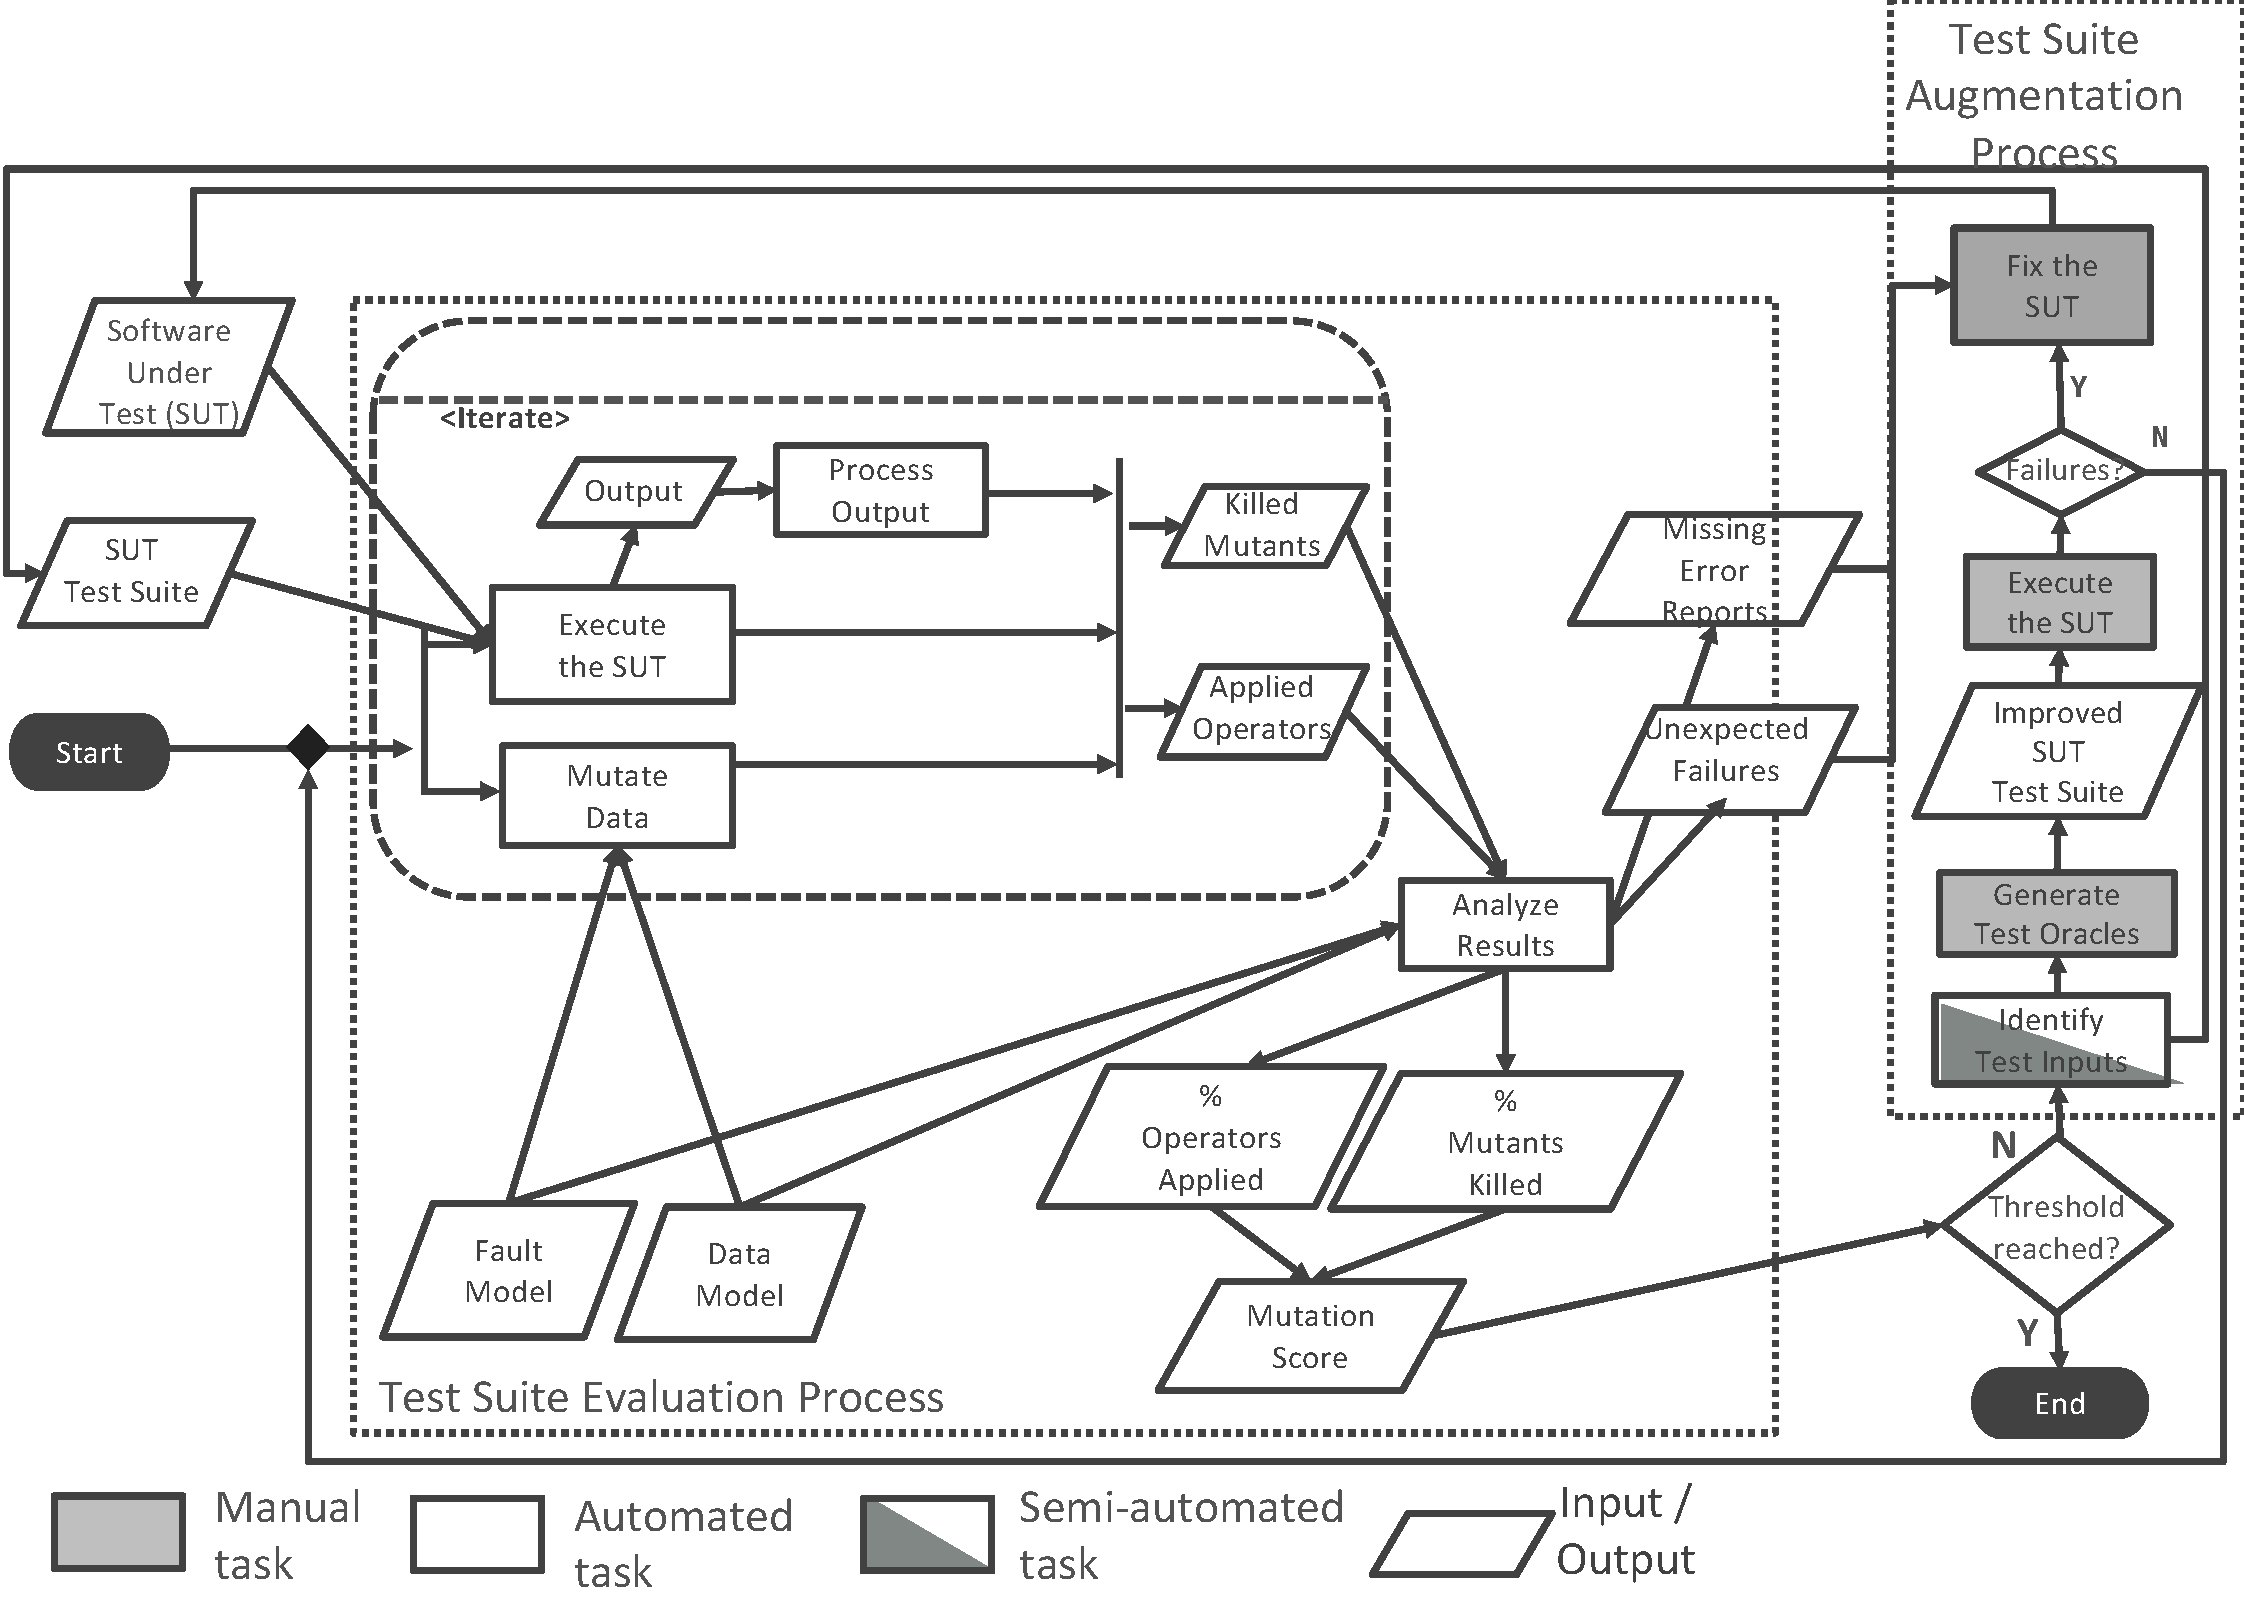
\includegraphics[width=\textwidth]{images/dataProcess}
		\caption{Data-driven Mutation Testing Process.}
		\label{fig:data:process}
	\end{figure}



This Chapter defines a test suite assessment process based on the injection of faults in the data processed by software components; we refer to this process as \INDEX{data-driven mutation testing}. 
%The definition of data-driven mutation testing is a unique contribution of this book; it has not been presented in previous literature work.

Data-driven mutation testing aims to assess test suites by simulating faults that affect the data produced, received, or exchanged by the software and its components.
It is based on a \INDEX{fault model} capturing the type of data faults that might affect the system. The fault model is produced by software engineers based on their domain knowledge and experience~\cite{di2015generating}. The considered faults might be due to programming errors, hardware problems, or critical situations in the environment (e.g., noise in the channel). The data is then automatically  mutated (i.e., modified) by a set of operators that aim to replicate the faults in the fault model. For example, the \INDEX{bit flip operator} flips a randomly selected bit of a field of the transmitted data (see Section~\ref{sec:faultModel}). 
%Mutation operators can be applied multiple times, on different data chunks or over repeated executions of a test case, ti


Figure \ref{fig:data:process} shows the reference data-driven mutation testing process that will be considered in FAQAS. The process is based on two main sub-processes, \EMPH{test suite evaluation} and \EMPH{test suite augmentation}, which are described in Sections~\ref{sec:data:test_suite_evaluation}~and~\ref{sec:data:test_suite_augmentation}, respectively. Differently from the code-driven mutation testing process introduced in Section~\ref{sec:process}, the data-driven mutation testing process has not been formalized by existing software testing literature. An extensive discussion of related work has been presented in deliverable D1.

\MREVISION{C-P-29}{The type of faults that might be simulated by data-driven mutation testing are CPU faults, memory faults, data processing faults, and communication faults. 
However, it is worth noting that these faults are the means to perform mutation testing (i.e., evaluate test suites), they are not the purpose of data-driven mutation testing. Data-driven mutation testing does not aim at simulating such faults to determine if the system is robust but it aims to determine if, in the presence of such faults, the test suite fails as it would be expected. The choice of the faults to simulate depends on the type of test suite to evaluate.}

\CHANGED{In FAQAS we focus on evaluating the quality of functional test suites. In the following, we briefly discuss the reasons why we do not evaluate robustness testing test suites, which, among the different types of test suites, is the closest to mutation testing. Indeed,  it is often performed through mutation.
Space systems are expected to be robust with respect to CPU faults and memory faults; for this reasons such faults are often the means for performing robustness testing. Robustness testing is often performed by relying on ad-hoc fault injection systems (e.g., by corrupting memory through debugger features), which may require the test cases to be manual performed. For these reasons evaluating the quality of robustness test cases with an automated and generic strategy appear infeasible.}

%\CHANGED{To perform data-driven mutation testing of functional test suites all the different types of faults might be considered (e.g., CPU faults, memory faults, data processing faults, and communication faults). However, CPU faults and memory faults simply result into erroneous results, which are simulated by replacing valid values or performing bit flips.}

\CHANGED{With data-driven mutation testing we aim to simulate higher-level problems that typically affect complex data structures. The main reason is that other types of problems (e.g., computation of erronous results) are already targeted by code-driven mutation. For this reason, we aim to perform data-driven mutation testing at the boundary of software components.
An ideal target for data-driven mutation testing are loosely coupled software components; typically the ones that run on separated pieces of hardware (e.g., the on board controller and the ADCS).
Despite other cases can be envisaged (e.g., pure software components that run on the same hardware), we target components running on separated hardware since we believe they are more likely affected by problems due to an incorrect understanding of requirements specifications or error-handling (e.g., because developed by separate teams).}
%Since data-driven mutation testing alters the data produced, received, or exchanged by the software or its components, 

\CHANGED{For this reason, in FAQAS, we apply data-driven mutation testing to evaluate test suites that trigger the execution and communication between multiple components (e.g., system or integration test cases). In FAQAS, data-driven mutation testing is not meant to be applied to assess unit test suites.}

\clearpage
\section{Test Suite Evaluation} % (fold)
\label{sec:data:test_suite_evaluation}

The test suite evaluation process consists of three activities \EMPH{Execute the SUT}, \EMPH{Mutate Data},  and \EMPH{Analyze Results}.
The activity \INDEX{Execute the SUT} indicates that the SUT is executed against its automated test suite. 
The activity \INDEX{Mutate Data} concerns the automated modification of either the data received by the software, the data produced by the software, or the data exchanged by software components.
In Figure~\ref{fig:data:process}, the activity \EMPH{Mutate Data} is executed in parallel to the activity \EMPH{Execute the SUT} since data modification should occur at runtime during test cases execution, to simulate software faults affecting the data processed by the software.



%The fault model enables engineers to minimize the presence of equivalent mutants.
%The data model may capture the relation between inputs and outputs of the system

\begin{figure}
	\centering
		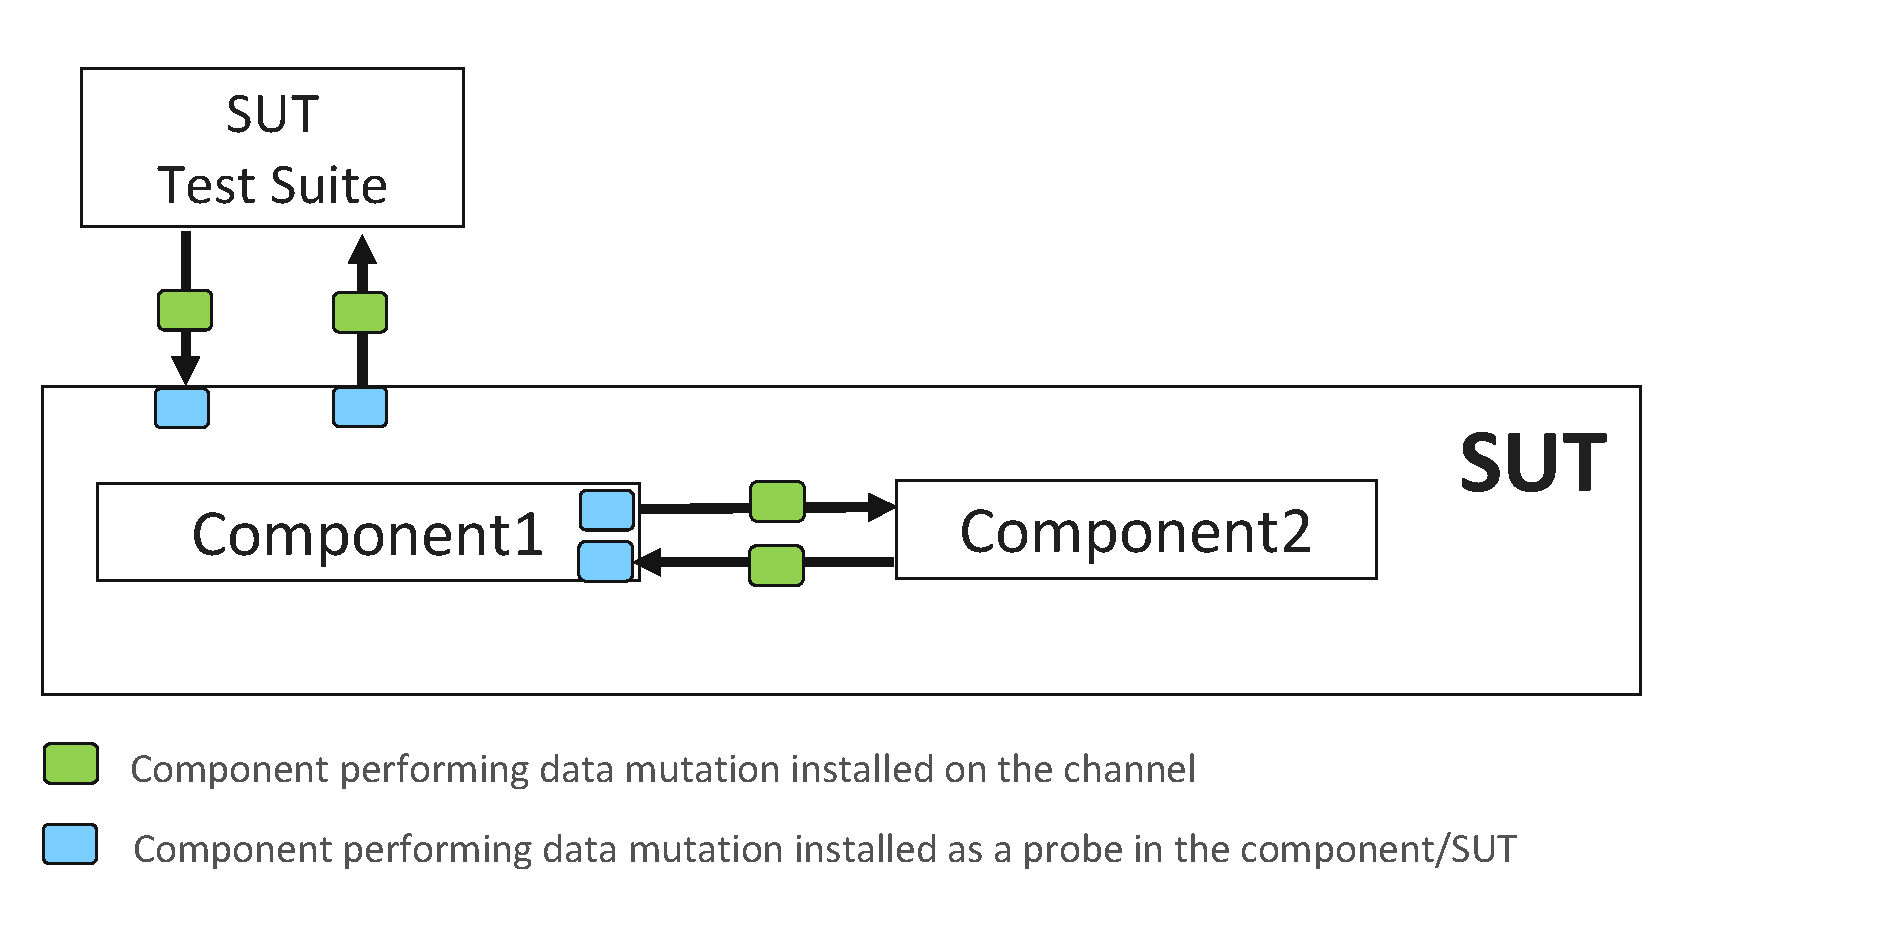
\includegraphics[width=10cm]{images/dataMutationExample}
		\caption{Example of implementation of a data mutation solution.}
		\label{fig:data:mutateData}
	\end{figure}
	
Figure~\ref{fig:data:mutateData} provides an example of how the Mutate Data activity can be implemented. Figure~\ref{fig:data:mutateData} shows that, to implement data mutation, it is necessary to integrate additional components that alter the data exchanged by the SUT components at runtime on a certain communication layer. We call such components \INDEX{mutation probes}.

%Since an ideal target for data-driven mutation testing is the communication between loosely coupled software components; typically the ones that run on separated pieces of hardware (e.g., the on board controller and the ADCS).

\MREVISION{C-P-31}{The communication between loosely coupled software components is performed by relying on APIs of a dedicated communication layer; which is typical in well designed software systems.
The functioning of such communication layer may vary from system to system. The communication layer works by serializing and deserializing the data that should be transmitted on the communication channel. The goal of serialization/deserialization is to perform a data transformation, i.e, translate the representation of data from the format used inside the program (e.g., a data structure) into a low level format that can be transmitted on the channel (e.g., a stream of bytes or a memory buffer).}

\CHANGED{The differences that we may observe from system to system are related to the input interface of the communication layer. We may observe two cases:}

\CHANGED{\begin{itemize}
\item The communication layer provides serialization (deserialization) primitives that receive (produce) unstructured data (e.g, a memory buffer).
\item The communication layer provides serialization (deserialization) primitives that receive (produce) data structured according to a specific format. 
\end{itemize}}

\CHANGED{In both the two cases, the communication layer performs a data transformation, i.e, translates the data from the format used inside the program (e.g., a data structure) into a low level format that can be transmitted on the channel (e.g., a memory buffer). However, this commonality does not enable the definition of a single solution to perform data mutation. More precisely, \EMPH{a solution that performs mutation on memory buffers may not be practical in both the two cases}. Indeed, to alter data that is already flattened on a low level representation it is necessary a (potentially complex) data model that describes how to load such data into a more structured representation that should drive the mutation. 
The data modelling effort would thus be redundant in case the data is structured according to a specific format.} 

\CHANGED{To minimize modelling costs, in the presence of a complex data structure, the data model should coincide with the data structure defined in the programming language used to implement the system (or the modelling language from which the program has been derived), while the fault model should be defined as an extension of such data structure (e.g., through annotations).
Modelling of data flattened into a low level representation is feasible only when this is already the input format of the communication layer (in such cases the transmitted data is not expected to follow a complex structure).
Finally, the definition of a generic data loading solution 
that loads data from a memory buffer into a more structured representation and works with any data structure, might be infeasible. 
%structures (e.g, fields of variable size and multiple dependencies among fields), 
%might be particularly expensive.
}

\CHANGED{In FAQAS case studies, the communication layer is either implemented in-house by the company that produced the case study or it is built by relying on the ASN.1 compiler architecture. In both the two cases, the communication layer implements distinct functions to serialize and deserialize data.
However, in the case of in-house communication layer, the system work by processing a flat structure, while in the case of the ASN.1 compiler architecture the data processed by the compiler is highly structured. The definition of the data structure is provided as an ASN.1 grammar that is then translated by the ASN.1 compiler into a C structure. For this reason, \EMPH{in FAQAS, we propose a solution for flat data stored in memory buffers and a solution for highly structured data defined with ASN.1}. Even if the ASN.1 data is translated into a C structure, we believe that a generic solution that rely on data models defined according to C structures might not be feasible. Indeed, data structures may contain elements with complex dependencies. For example, a tree data structure may define the tree depth  in a specific data field and programmers may assume that pointer to child nodes are not read when the max depth is not reached (i.e., pointer child pointers in leaf nodes are not NULL). Specifying such logic into a generic framework is particularly hard if not infeasible.}

Concerning mutation probes, we expect them to be \EMPH{integrated into the software API functions that either serialize or deserialize the data being sent on the communication channel}.

In the case of a communication layer implemented in-house, we expect mutation probes to be integrated into the software under test by engineers who \EMPH{manually} add calls to the functions of a \INDEX{data-driven mutation testing API} in the source code of the software. Indeed, since communication APIs vary from system to system, it is not possible to define a tool that automatically modifies the source code or the executable code of the SUT.  Instead, we provide a \INDEX{data-driven mutation testing API} that implements the logic for mutating the data specified by the engineer.
To be applicable to a wide range of software systems, the API will provide methods that enable mutating data buffers provided as C arrays.
Figure~\ref{fig:data:mutationProbes} shows an example of a mutation probe manually integrated into the source code (API method names begin with the prefix \emph{\_FAQAS}).

In the case of a communication layer implemented by relying on the ASN.1 compiler, the FAQAS framework will automatically introduce mutation probes into the code that \CHANGED{serializes/deserializes data.}




\begin{figure}
	\centering
		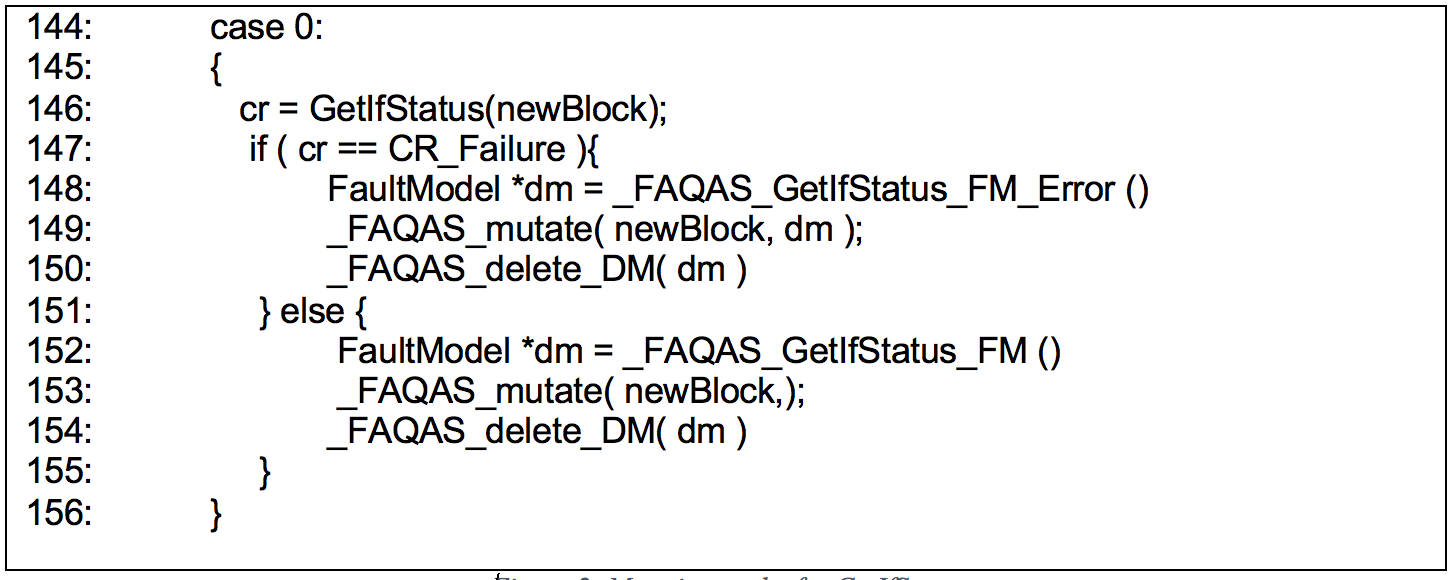
\includegraphics[width=10cm]{images/dataMutationProbes}
		\caption{Example of integration of data mutation probes.}
		\label{fig:data:mutationProbes}
	\end{figure}

%\TODO{ADD concrete example of integration}

	
%Data-driven mutation testing is driven by a faulty model specifying how to alter the data (i.e., the attributes declared in an ASN.1 grammar or the array items).	
In deliverable D1, we have clarified that, in a generic data-driven mutation testing process, the activity \EMPH{Mutate Data} may require a \INDEX{data model} that captures the characteristics and structure of the data to be mutated. 
The data model should be used to load a stream of bytes in structured form (e.g., an instance of a given data structure), which is necessary to drive data mutation. 
Also, the activity \EMPH{Mutate Data} should be driven by a \INDEX{fault model} that specifies the set of mutation operators to apply~\cite{di2015generating}. 
In FAQAS, the data model and the fault model are coupled into a same structured representation, i.e., the \INDEX{FAQAS fault model}, which is presented in Section~\ref{sec:faultModel}.


The activities \EMPH{Execute the SUT} and \EMPH{Mutate Data} are repeated till all the faults of the fault model had been applied. The possible stopping criteria are described in Section~\ref{sec:mutantsExecution}. 

The activity \INDEX{Process Outputs} processes all the outputs generated during the execution of test cases.
The collected outputs include the result of test cases execution (i.e., the list of test cases that either passed or failed) and the logs generated by the SUT during testing.
In the context of data-driven mutation testing both the \INDEX{test results} and the \INDEX{log files} are necessary to determine if a test suite kills a mutant.
Indeed, \emph{in the context of data-driven mutation testing a mutant is killed either if a test case fails, or if the software activates robustness features capable of handling the specific data fault.}
We need log files to determine if robustness features had been triggered.
For example, a system that implements a \INDEX{robust communication protocol} might simply request again the packets affected by errors thus avoiding failures. In this case, we need to inspect the log files to determine if the robustness feature had been triggered.
The fault model is expected to include only data fault classes that should either lead to failures or make the system generate an error entry in the log file.

Differently from code-driven mutation testing, data-driven mutation testing does not alter the software implementation but only the data processed by software components, for this reason it may help engineers to \INDEX{identify existing faults}, an objective that cannot be achieved by code-driven mutation testing. 
This is the case when \emph{Missing Error Reports} or \emph{Unexpected Failures }(e.g, crashes) are observed. In both the two cases, engineers should fix the system. In code-driven mutation testing, faults can be detected only after introducing new test cases that kill the generated mutants.

The activity \INDEX{Analyze Results} provides an assessment of the quality of the test suite for the SUT.
It is driven by two objectives:
\begin{itemize}
\item[(O1)] determine if the test suite is capable of detecting software faults that affect the data processed by the software components 
(e.g., we expect a test suite to fail in case the data exchanged by two components contains invalid values).
\item[(O2)] determine if the test suite exercises enough software behaviours to discover all the possible faults that may affect the data produced by the system
(i.e., it should be possible to alter the processed data to generate faulty data according to the fault model). 
\end{itemize}

Objectives O1 and O2 are complementary, they both should be addressed by data mutation.
For example, a use case scenario for data-driven mutation testing could be the following: (i) data-driven mutation testing is applied to the data exchanged by \emph{component 1} and \emph{component 2} in Figure~\ref{fig:data:mutateData}, (ii) the data exchanged by the two components follow the data model in Figure~\ref{fig:DataDrivenSimpleExample}, and (iii) mutation testing is performed by applying the bit-flip mutation operator to every field of the messages being exchanged.
The data model in Figure~\ref{fig:DataDrivenSimpleExample} consists of a UML class diagram that indicates that the two components can send messages whose type can be either \emph{TimeMessage} or \emph{DataMessage}. A \emph{TimeMessage} contains only one field of type Long, which is the timestamp. 
A \emph{DataMessage} contains two fields, one field of type \emph{Integer} capturing the size of the payload, and one array of bytes containing the payload. 
Objective O1 is fulfilled when every mutant leads to the failure of least one test case.
Objective O2 is fulfilled when mutation testing generates at least (i) one \emph{TimeMessage} with field \emph{timestamp} being altered,
(ii) one \emph{DataMessage} with field \emph{size} being altered,
and (iii) one \emph{DataMessage} with field \emph{payload} being altered.
For a test suite consisting of two test cases that trigger the exchange of the messages as in the bottom-left part of Figure~\ref{fig:DataDrivenSimpleExample}, the execution of the bit flip mutation operator may lead to messages that lead to test failures. Since all the mutants are killed (i.e., the two test cases fail), objective O1 is achieved. However, the test suite does not lead to the exchange of any message of type \emph{DataMessage}, for this reason objective O2 is not achieved. Objective O2 enables us to determine that the test suite does not exercise the case in which the two components exchange messages of type \emph{DataMessage}. When data-driven mutation testing is performed against components that are expected to guarantee robustness against the exchange of erroneous data, as a by-product, objective O2 also ensures that components' robustness is properly tested.



\REVTWO{C34}{Activity \emph{Analyze Results} concerns the automated computation of the \INDEX{mutation score} from execution data. It is 
computed as the weighted average of the percentage of mutants being killed and the percentage of mutation operators applied.}
The former enables data-driven mutation to achieve objective O1, the latter objective O2. 
%Details are provided in Section~\ref{sec:data:mutationscore}.

\REVTWO{C34}{Activity \emph{Analyze Results} takes as input the the data model, the fault model, the list of killed mutants, and the list of mutation operators applied.}
The list of applied mutation operators should enable engineers to determine if all the available mutation operators have been applied.


\begin{figure}[t!]
  \centering
    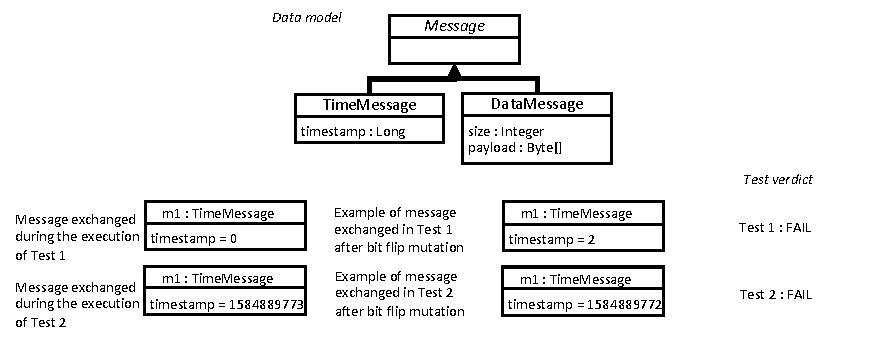
\includegraphics{images/DataDrivenSimpleExample}
      \caption{Simplified data mutation example.}
      \label{fig:DataDrivenSimpleExample}
\end{figure}

\clearpage



\clearpage
\subsection{FAQAS Fault Model}
\label{sec:dataModel}
\label{sec:faultModel}





A building block of the fault model are a set of \EMPH{data fault classes}.
A  \INDEX{data fault class} captures the type of an error that might affect the data. In turns, it specifies the mutation that should be applied in order to replace valid data with erroneous data. For each fault class we have defined a corresponding \INDEX{data mutation operator} having the same name. 
Each {data mutation operator} performs data mutation by applying a \INDEX{data mutation operation} (e.g., set a value above the upper range value). Mutation operators might apply one or more data mutation operations.
Each data mutation operator can be configured with a set of parameters. 

Table~\ref{table:faultModel:FAQAS} provides a preliminary list of data fault classes that will be supported by the FAQAS framework along with a description. For each fault class we indicate the data types to which it is expected to be applied, we identify \FIXME{six} data types: 
\begin{itemize}
\item int, which indicates an integer 
\item long int, which indicates a long integer 
\item float, which indicates a floating point number
\item double, which indicates a double precision floating point number
\item bin, which indicates data that should be treated in its binary form
%\item hex, which stands for an hexadecimal value
\item array[x], which stands for an array of $x$ variables of a given type. In our implementation, the value $x$ might be a number or, for arrays of variable size, a reference to the i-th field in the data buffer, which is supposed to contain the array size\footnote{In our implementation, we specify a negative value to determine that the value of $x$ refers to the x-th variable}.  The array type is specified in the array type name. More precisely, the engineer should provide a specific keyword that consists of the keyword 'array' followed by the name of the primitive type, as follows:
\begin{itemize}
\item array\_int
\item array\_long\_int
\item array\_float
\item array\_double
\item array\_bin
%\item array\_hex
\end{itemize}
\end{itemize}

\CHANGEDNOV{We believe that the technology implementing data mutation should depend on the type of system under test. This is mostly due to the need for (1) implementing mutation operations that are fast and (2) reducing the amount of data-modelling to be manually performed (ideally engineers would like to reuse existing models and artefacts). Based on the case studies shared for WP2, we observe that data-driven mutation testing might be performed by modifying either data that is stored in an array or in a data structure defined through the ASN.1 grammar. In our vision, these two solutions differ for the strategy used to model the data and for the algorithms implemented to execute mutation. Despite a more general solution (e.g., based on UML models) that glue together these two strategies might be feasible, its implementation might be the target of an ESA activity. Indeed, when data modelling is based on generic high-level models it is necessary to implement a layer that translate high-level representation into low-level data that can be efficiently processed at runtime. The following subsections describe the two distinct cases; however, in FAQAS, we will focus on the implementation of a solution for buffer arrays. The main reasons are two (1) buffer arrays appear to be a common strategy for implementing data communication (2) in FAQAS we lack case studies based on the ASN.1 grammar (see Section~\ref{sec:caseStudies:ASN:data}).}







% !TEX root = ../MAIN.tex
\begin{table}[h]
\begin{center}
\scriptsize
\begin{tabular}{|p{2cm}|p{2cm}|p{4cm}|p{6cm}|}
\hline
\textbf{Fault Class}&\textbf{Types}&\textbf{Parameters}&\textbf{Description}\\
\hline
Value above threshold (VAT)&
\begin{minipage}{6cm}
INT\\
LONG INT\\
FLOAT\\
DOUBLE
\end{minipage}
&
\begin{minipage}{6cm}
T: threshold\\
D: delta with respect to threshold\\
\end{minipage}
&
\begin{minipage}{6cm}
The value is above a threshold T for a delta D. 

\EMPH{Data mutation operation:} The mutation is performed by replacing the current value (a number) with a value of the same type that is equal to $(T+D)$.
\end{minipage}
\\

\hline
Value below threshold (VBT)&
\begin{minipage}{6cm}
INT\\
LONG INT\\
FLOAT\\
DOUBLE
\end{minipage}
&
\begin{minipage}{6cm}
T: threshold\\
D: delta with respect to threshold\\
\end{minipage}
&
\begin{minipage}{6cm}
The value is below a threshold T for a delta D. 

\EMPH{Data mutation operation:} The mutation is performed by replacing the current value (a number) with a value of the same type that is equal to $(T-D)$.
\end{minipage}
\\



\hline
Value out of range (VOR)&
\begin{minipage}{4cm}
INT\\
LONG INT\\
FLOAT\\
DOUBLE
\end{minipage}
&
\begin{minipage}{4cm}
MIN: minimum valid value\\
MAX: maximum valid value\\
D: delta with respect to minimum/maximum valid value
\end{minipage}
&
\begin{minipage}{6cm}
The value is out of the valid range MIN-MAX. 

\EMPH{Data mutation operations (2):}  The mutation is performed by replacing the current value (a number) with 
\begin{itemize}
\item a value of the same type that is equal to $(MIN-D)$
\item a value of the same type that is equal to $(MAX+D)$
\end{itemize}
\end{minipage}
\\

\hline
Bit flip (BF)&
BIN
&
\begin{minipage}{4cm}
MIN: lower bit\\
MAX: higher bit\\
STATE: mutate only if the bit is in the given state\\
\TRFOUR{VALUE: integer specifying the number of bits to mutate}\\
\end{minipage}
&
\begin{minipage}{6cm}
A number of bits randomly chosen in the positions between MIN and MAX (included) are flipped.

\EMPH{Data mutation operation:} the operator flips N randomly selected bit.
If STATE is specified, the mutation is applied only if  the bit is in the specified state. Parameter VALUE specifies the number of bits to mutate.
\end{minipage}
\\

\hline
Invalid numeric value (INV)&
\begin{minipage}{6cm}
INT\\
LONG INT\\
FLOAT\\
DOUBLE
\end{minipage}
&
\begin{minipage}{4cm}
MIN: lower valid value\\
MAX: higher valid value\\
\TRFOUR{D: distribution to follow}\\
\TRFOUR{VALUE: mean value for normal distribution}\\
\end{minipage}
&
\begin{minipage}{6cm}
The value is legal (i.e., in the specified range) but different than the current one, which, in this case, is expected to be consistent with the status of the system.

\EMPH{Data mutation operation:} Mutation is performed by replacing the current value with a different value randomly sampled in the specified range. The parameter D specified the distribution to follow when performing the mutation\footnote{In our implementation 0 indicates uniform, 1 indicates normal around the specified value (but in range).}
\end{minipage}
\\

\hline
Illegal Value (IV)
&
\begin{minipage}{6cm}
INT\\
LONG INT\\
FLOAT\\
DOUBLE
\end{minipage}
&
\begin{minipage}{6cm}
VALUE: illegal value that is observed\\
\end{minipage}
&
\begin{minipage}{6cm}
The value is illegal and equal to the provided one (i.e., parameter \emph{VALUE}).

\EMPH{Data mutation operation:} Mutation is performed by replacing the current value with the value \emph{VALUE}, if different than the current one.
\end{minipage}
\\

\hline
\TRFOUR{Anomalous Signal Amplitude (ASA)}
&
\begin{minipage}{6cm}
INT\\
LONG INT\\
FLOAT\\
DOUBLE
\end{minipage}
&
\begin{minipage}{6cm}
T: change point\\
D: delta to add/remove\\
V: value to multiply\\
\end{minipage}
&
\begin{minipage}{6cm}
The value is modified by amplifying/reducing it by a factor V and adding or removing D from the observed value. It is used to "amplify" a signal in a constant manner to simulate unusual signal. T indicates the observed value below which instead of adding  we subtract .

\EMPH{Data mutation operation:} Mutation is performed by replacing the current value ($v$) with the value ($v'$) computed as follows:

\[
v' =  
    \begin{cases}
      T+(  (v-T)*V  ) + D   & \mathit{if}\ v \ge T\\
      T - (  (T-v)*V  ) - D   & \mathit{if}\ v < T
    \end{cases}       
\]
\end{minipage}
\\


\hline
\TRFOUR{Signal Shift (SS)}
&
\begin{minipage}{6cm}
INT\\
LONG INT\\
FLOAT\\
DOUBLE
\end{minipage}
&
\begin{minipage}{6cm}
D: delta by which the signal should be shifted\\
\end{minipage}
&
\begin{minipage}{6cm}
The value is modified by adding a value D. It simulate an anomalous shift in the signal.
\end{minipage}
\\





\hline
\TRFOUR{Hold Value (HV)}
&
\begin{minipage}{6cm}
BIN\\
INT\\
LONG INT\\
FLOAT\\
DOUBLE
\end{minipage}
&
\begin{minipage}{6cm}
V: number of times to repeat the same value\\
\end{minipage}
&
\begin{minipage}{6cm}
This operator keeps repeating an observed value for $V$ times. It emulates a constant signal replacing a signal supposed to vary.
\end{minipage}
\\



\hline
\TRFOUR{Array Swap (AS)}
&
\begin{minipage}{6cm}
ARRAY\_*\\
\end{minipage}
&
\begin{minipage}{6cm}
MIN: position of element A\\
MAX: position of element B\\
VALUE: number of elements to move\\
\end{minipage}
&
\begin{minipage}{6cm}
Replace a number of elements (number specified by VALUE) located starting from position MIN, with a number of elements located starting from position MAX, and viceversa.
\EMPH{Data mutation operation:} Mutation is performed by replacing the two set of elements with each other.
\end{minipage}
\\


\hline
\TRFOUR{Array Random Swap (ARS)}
&
\begin{minipage}{6cm}
ARRAY\_*\\
\end{minipage}
&
\begin{minipage}{6cm}
MIN: min position of element A/B\\
MAX: max position of element A/B\\
VALUE: number of elements to move\\
\end{minipage}
&
\begin{minipage}{6cm}
Replace a number of elements (number specified by VALUE) located in a position between MIN and MAX, with a number of elements located in a position between MIN and MAX. MIN and MAX specify a position with respect to the beginning and end of the array.  For example, MIN=0 indicates the first element of teh array, MIN=-2 indicates the second element of the array.
\EMPH{Data mutation operation:} Mutation is performed by replacing the two set of elements with each other.
\end{minipage}
\\



%Incorrect Identifier& Several transmission data fields have fixed values, for example fields identifying the transmitting satellite. Hardware/software errors may assign incorrect identifiers.\\
%%Incorrect Checksum& Hardware/software errors may result in an incorrect checksum for a Packet or VCDU.\\
%Incorrect Counter& Counters are used to track Packet or VCDU ordering. Hardware/software errors may assign incorrect counter values.\\
%Flipped Data Bits& Physical channel noise may flip one or more bits in the data transmission.\\
\hline
\end{tabular}
\end{center}
\caption{Data Fault Classes}
\label{table:faultModel:FAQAS}
\end{table}%

\clearpage

\subsubsection{Fault Model Specifications for Data Buffers}

When the data to be mutated is stored in an array, we require the definition of a fault model in the form of a block diagram, i.e., by specifying the data type of a sequence of data items. We rely on this format because it enables to represent the sequence of data items in the buffer (array) used by the communication APIs.
 
For each data item, the FAQAS fault model captures its \EMPH{type} and a list of \INDEX{data fault classes} that might affect the item. 
The type of the data item indicates how the values of the bits in the data item should be interpreted (e.g., as a floating point number). Since a data type may span over multiple items of the data buffer, for each block, we may indicate whether also the values of the following blocks should be used to load the data.

Table~\ref{table:faultModel:example} provides an example of two fault models described in tabular form. 
It resembles the CSV format supported by the FAQAS toolset. For each data item we report the span, type, and fault class. For each fault class we indicate the values of the configuration parameters for the corresponding mutation operator. The fault model \EMPH{IfHK} leads to five mutation operation instances: one for each of the two BF mutation operators, one for the VAR operator, and two for the VOR mutation operator. The fault model characterizes an array of five elements containing four data items; all the data items occupy one array element except for the third data item (i.e., the data item with ID 2), which occupies two array positions (span is equal to 2).

Figure~\ref{fig:dataMutationFMExamples} provides a visual representation of an array of 8 bit unsigned integers (i.e., unsigned chars) that is modelled using the \EMPH{IfHK} fault model in Table~\ref{table:faultModel:example}. It also provides an example of the mutated data generated by the six mutation operation instances derived from the fault model in Table~\ref{table:faultModel:example}.


% !TEX root = ../MAIN.tex
\begin{table}[h]
\begin{center}
\small
\begin{tabular}{|p{1cm}|p{2cm}|p{1cm}|p{1cm}|p{1cm}|p{1cm}|p{1cm}|p{2cm}|p{1cm}|p{1cm}|}
\hline
\textbf{Fault Model Name}&\textbf{DataItem}&\textbf{Span}&\textbf{Type}&\textbf{Fault Class}&\textbf{Min}&\textbf{Max}&\textbf{Threshold}&\textbf{Delta}&\textbf{State}\\
\hline
IfHK&0&1&BIN&BF&0&0&-&-&-\\
IfHK&1&1&INT&VOR&0&5&-&1&-\\
IfHK&2&2&BIN&BF&0&63&-&-&-\\
IfHK&4&1&BIN&BF&0&0&-&-&-\\
\hline
IfStatus&0&1&BIN&BF&0&0&-&-&-\\
\hline
\end{tabular}
\end{center}
\caption{Driven Fault Model Buffer}
\label{table:faultModel:example}
\end{table}%

\begin{figure}[h]
  \centering
    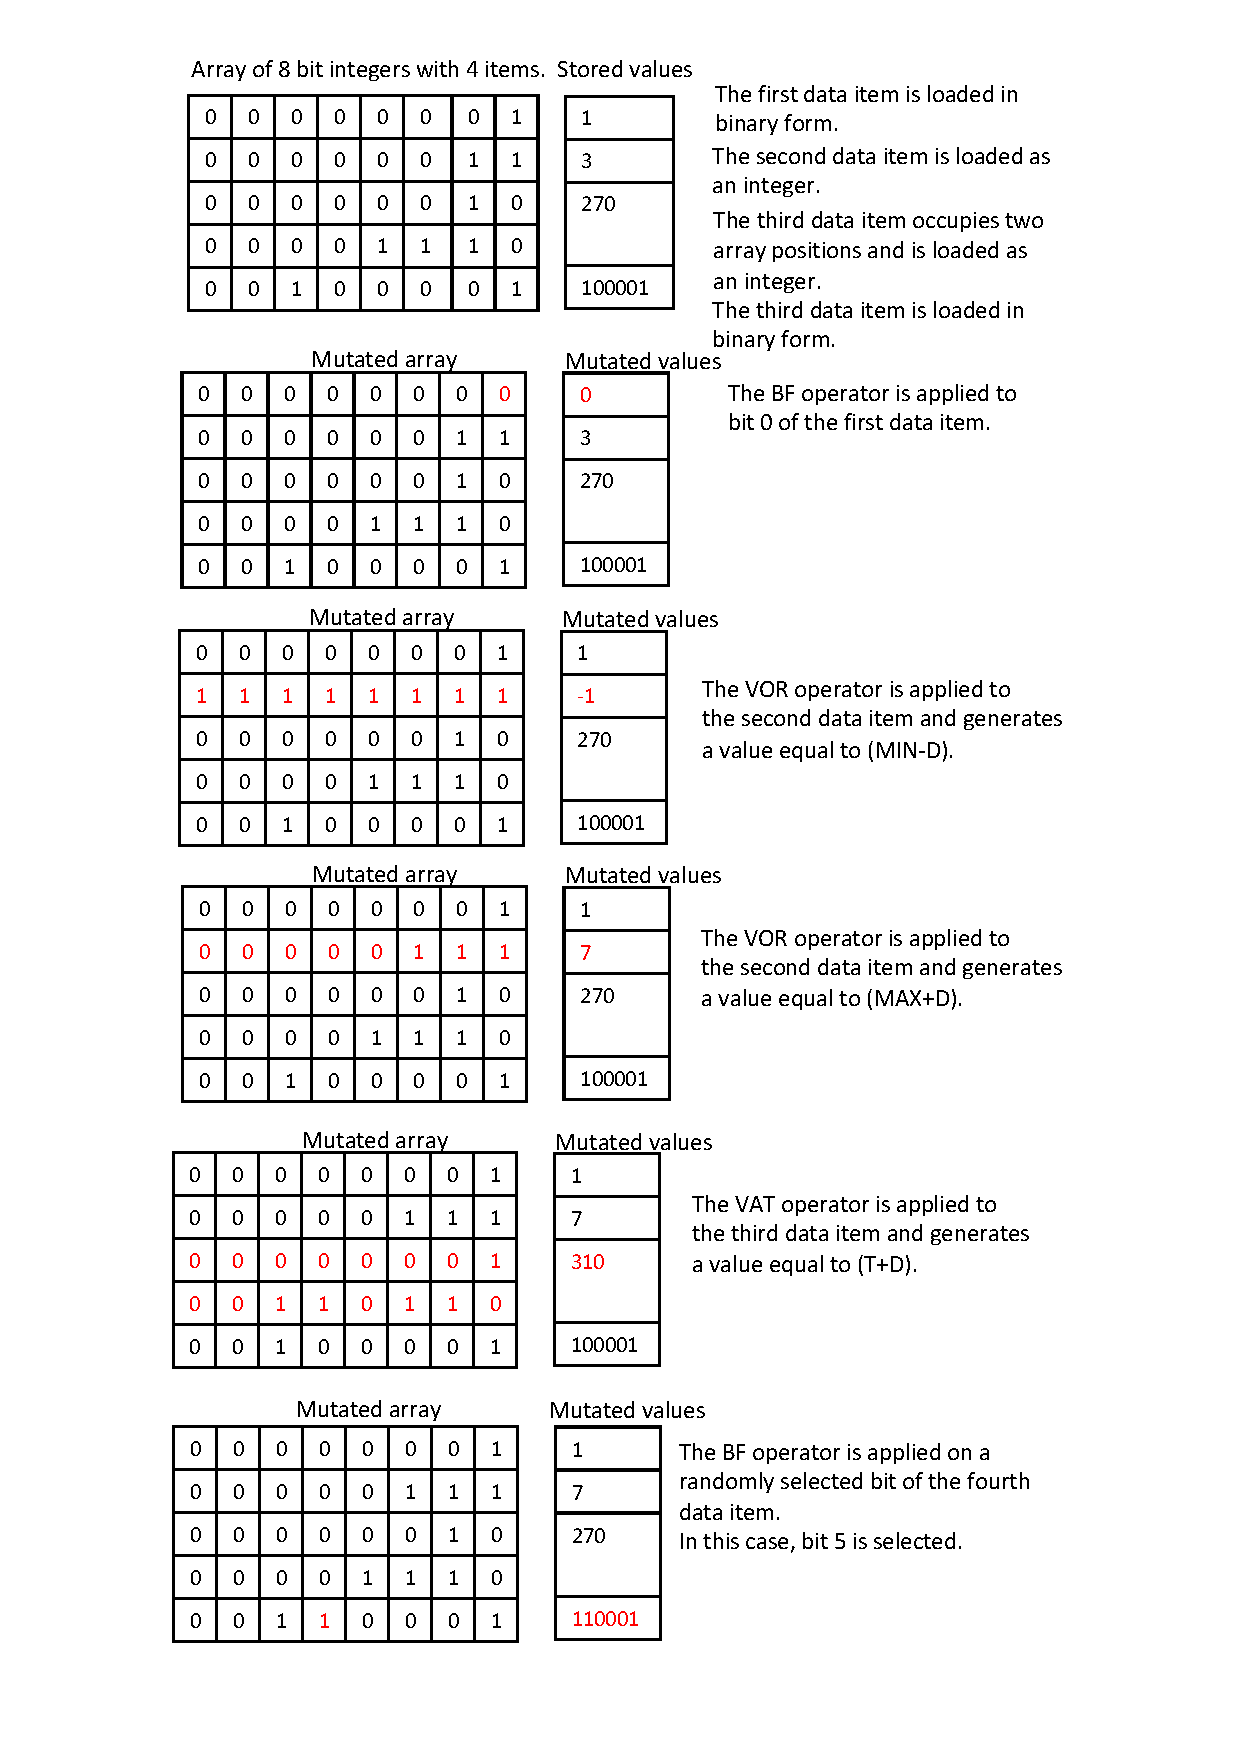
\includegraphics[width=12cm]{images/dataMutationFMExample.pdf}
      \caption{Example of original data and  data mutated according to the fault model in Table~\ref{table:faultModel:example}.}
      \label{fig:dataMutationFMExamples}
\end{figure}

\clearpage
\subsubsection{Fault Model Specifications for ASN.1 grammar}
\label{subsub:asn1model}

The ASN.1 grammar enables engineers to specify data structures where the types of the items in the data structure are selected from a predefined set.

%When the data to be mutated is stored in a data structure defined through the ASN.1 grammar, the fault model is specified by indicating which operators to apply on the specific fields of the data structure. 

We have identified a set of feasible fault classes for each type supported by the ASN1CC compiler.
The corresponding mutation operators are automatically configured based on the ASN.1 grammar (e.g., in the case of an attribute of type INTEGER, the min/max values of the VOR operator are derived from the boundaries of the INTEGER type).
Table~\ref{table:faultModel:FAQAS:ASN1} provides, for each of such types, the feasible fault classes and the configurations for the mutation operators.
In the configuration for the mutation operators, we refer to the variables (e.g., MIN and MAX) appearing in the ASN.1 xml file.

Figure~\ref{fig:ASN1ProbesGeneration} provides an overview of the process in place to generate probes including the fault model.
The engineer first export the ASN.1 grammar as XML, then he modifies the generated file by specifying, for each \emph{Asn1Type}, the mutation operator to be used (this is done by adding an xml attribute called \emph{MutationOperator} with a value specifying the name of the operator). 

An example is provided in Listings~\ref{asnXML} and \ref{asnXMLUpdated}. Listing~\ref{asnXML} provides the xml generated by the grammar, which includes two INTEGER types.
Listing~\ref{asnXMLUpdated} provides the xml updated by the engineer, who indicates that the two integers should be mutated with the VAR and the VOR operator. To tune the operators, the engineer updates the MIN and MAX values for those integers to capture only nominal values. 
In the case of the first integer (the one to be mutated with VAR), the engineer sets 5 as MAX.
In the case of the second integer (the one to be mutated with VOR), the engineer sets MIN and MAX to 0 and 50 respectively.
%The engineer can tune the mutation by changing the value ranges associated to the different types. For example, this could be done to restrict the valid range of an INTEGER from (MIN=-100, MAX=100) to a nominal range of (MIN=0,MAX=50).
In case a data type is defined through value range constraints, the FAQAS framework will configure one mutation operator instance for each range.

% !TEX root = ../MAIN.tex
\begin{table}[h]
\begin{center}
\small
\begin{tabular}{|p{2cm}|p{2cm}|p{4cm}|p{4cm}|}
\hline
\textbf{Types}&\textbf{Fault Classes}&\textbf{Parameters}&\textbf{Description}\\
\hline
INTEGER&
VAT&
\begin{minipage}{4cm}
T: MAX\\
D: 1\\
\end{minipage}
&
\begin{minipage}{4cm}
\end{minipage}
\\
\hline
INTEGER&
VBT&
\begin{minipage}{4cm}
T: MIN\\
D: 1\\
\end{minipage}
&
\begin{minipage}{4cm}
\end{minipage}
\\
\hline
INTEGER&
VOR&
\begin{minipage}{4cm}
MIN: MIN\\
MAX: MAX\\
D: 1\\
\end{minipage}
&
\begin{minipage}{4cm}
\end{minipage}
\\
\hline
REAL&
VAT&
\begin{minipage}{4cm}
T: MAX\\
D: 1\\
\end{minipage}
&
\begin{minipage}{4cm}
\end{minipage}
\\
\hline
REAL&
VBT&
\begin{minipage}{4cm}
T: MIN\\
D: 1\\
\end{minipage}
&
\begin{minipage}{4cm}
\end{minipage}
\\
\hline
REAL&
VOR&
\begin{minipage}{4cm}
MIN: MIN\\
MAX: MAX\\
D: 1\\
\end{minipage}
&
\begin{minipage}{4cm}
\end{minipage}
\\
\hline
ENUMERATED&
INV&
\begin{minipage}{4cm}
MIN: MIN\\
MAX: MAX\\
D: 1\\
\end{minipage}
&
\begin{minipage}{4cm}
\end{minipage}
\\
\hline
BOOLEAN&
BF&
\begin{minipage}{4cm}
MIN: 0\\
MAX: 0\\
\end{minipage}
&
\begin{minipage}{4cm}
\end{minipage}
\\
\hline
NULL&
BF&
\begin{minipage}{4cm}
MIN: 0\\
MAX: 0\\
\end{minipage}
&
\begin{minipage}{4cm}
\end{minipage}
\\
\hline
BIT STRING&
BF&
\begin{minipage}{4cm}
MIN: 0\\
MAX: 0\\
\end{minipage}
&
\begin{minipage}{4cm}
\end{minipage}
\\
\hline
OCTET STRING&
BF&
\begin{minipage}{4cm}
MIN: 0\\
MAX: 0\\
\end{minipage}
&
\begin{minipage}{4cm}
\end{minipage}
\\
\hline
IA5STRING&
BF&
\begin{minipage}{4cm}
MIN: 0\\
MAX: 0\\
\end{minipage}
&
\begin{minipage}{4cm}
\end{minipage}
\\
\hline
NUMERIC STRING&
BF&
\begin{minipage}{4cm}
MIN: 0\\
MAX: 0\\
\end{minipage}
&
\begin{minipage}{4cm}
\end{minipage}
\\
\hline
SEQUENCE&
-&
\begin{minipage}{4cm}
\end{minipage}
&
\begin{minipage}{4cm}
No mutation environed for this type.
\end{minipage}
\\
\hline
SET&
-&
\begin{minipage}{4cm}
\end{minipage}
&
\begin{minipage}{4cm}
No mutation environed for this type.
\end{minipage}
\\
\hline
CHOICE&
-&
\begin{minipage}{4cm}
\end{minipage}
&
\begin{minipage}{4cm}
No mutation environed for this type.
\end{minipage}
\\
\hline
SEQUENCE OF&
-&
\begin{minipage}{4cm}
\end{minipage}
&
\begin{minipage}{4cm}
No mutation environed for this type.
\end{minipage}
\\
\hline
SET OF&
-&
\begin{minipage}{4cm}
\end{minipage}
&
\begin{minipage}{4cm}
No mutation environed for this type.
\end{minipage}
\\



%Incorrect Identifier& Several transmission data fields have fixed values, for example fields identifying the transmitting satellite. Hardware/software errors may assign incorrect identifiers.\\
%%Incorrect Checksum& Hardware/software errors may result in an incorrect checksum for a Packet or VCDU.\\
%Incorrect Counter& Counters are used to track Packet or VCDU ordering. Hardware/software errors may assign incorrect counter values.\\
%Flipped Data Bits& Physical channel noise may flip one or more bits in the data transmission.\\
\hline
\end{tabular}
\end{center}
\caption{Data Fault Classes for ASN.1 data types.}
\label{table:faultModel:FAQAS:ASN1}
\end{table}%

Figure~\ref{fig:ASN1ProbesGeneration} shows that, finally, the FAQAS toolset generates a modified version of the ASN1 source code containing the serializer and deserializer functions. The generated source code contains the FAQAS API functions to mutate the data in ASN.1 data types. Examples are shown in the following sections (see Figure~\ref{ASN_mutations}).

\begin{figure}[h]
  \centering
    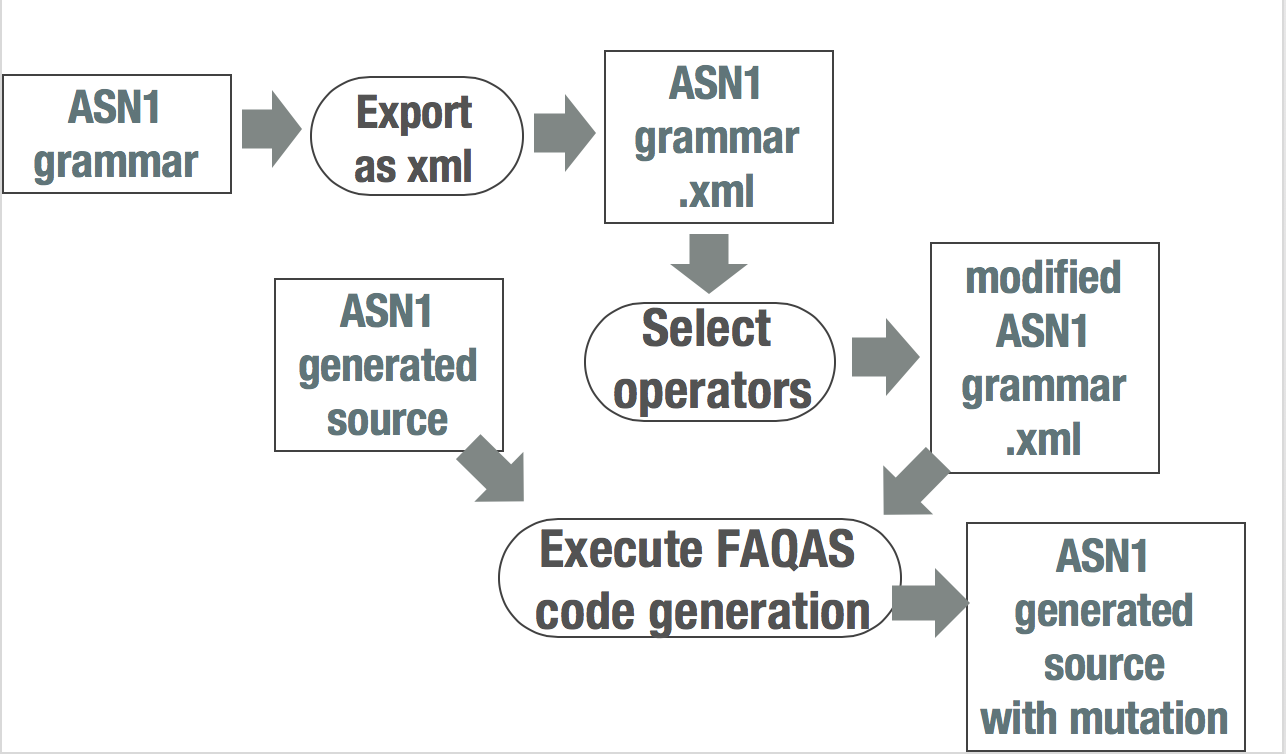
\includegraphics[width=12cm]{images/ASN1mutationProces}
      \caption{Data-driven probes generation process for ASN1.}
      \label{fig:ASN1ProbesGeneration}
\end{figure}


% !TEX root =  ../MAIN.tex

\begin{minipage}{15cm}
\begin{lstlisting}[style=CStyle, caption=Portion of an XML ASN1 grammar., label=asnXML, mathescape=true]
<TypeAssignment Name="TypeNested" CName="TypeNested" AdaName="TypeNested" Line="16" CharPositionInLine="0">
            <Asn1Type id="MY-MODULE.TypeNested" Line="16" CharPositionInLine="15" ParameterizedTypeInstance="false">
              <SEQUENCE acnMaxSizeInBits="3087" acnMinSizeInBits="2688" uperMaxSizeInBits="3087" uperMinSizeInBits="528">
                <SEQUENCE_COMPONENT Name="intVal" Line="17" CharPositionInLine="4" AdaName="intVal" CName="intVal">
                  <Asn1Type id="MY-MODULE.TypeNested.intVal" Line="17" CharPositionInLine="11" ParameterizedTypeInstance="false">
                    <INTEGER acnMaxSizeInBits="4" acnMinSizeInBits="4" uperMaxSizeInBits="4" uperMinSizeInBits="4">
                      <Constraints>
                        <Range>
                          <Min>
                            <IntegerValue>0</IntegerValue>
                          </Min>
                          <Max>
                            <IntegerValue>10</IntegerValue>
                          </Max>
                        </Range>
                      </Constraints>
                      <WithComponentConstraints />
                    </INTEGER>
                  </Asn1Type>
                </SEQUENCE_COMPONENT>
                <SEQUENCE_COMPONENT Name="int2Val" Line="18" CharPositionInLine="4" AdaName="int2Val" CName="int2Val">
                  <Asn1Type id="MY-MODULE.TypeNested.int2Val" Line="18" CharPositionInLine="12" ParameterizedTypeInstance="false">
                    <INTEGER acnMaxSizeInBits="5" acnMinSizeInBits="5" uperMaxSizeInBits="5" uperMinSizeInBits="5">
                      <Constraints>
                        <Range>
                          <Min>
                            <IntegerValue>-100</IntegerValue>
                          </Min>
                          <Max>
                            <IntegerValue>100</IntegerValue>
                          </Max>
                        </Range>
                      </Constraints>
                      <WithComponentConstraints />
                    </INTEGER>
                  </Asn1Type>
                </SEQUENCE_COMPONENT>
\end{lstlisting}
\end{minipage}


% !TEX root =  ../MAIN.tex

\begin{minipage}{15cm}
\begin{lstlisting}[style=CStyle, caption=Portion of an XML ASN1 grammar., label=asnXMLUpdated, mathescape=true]
<TypeAssignment Name="TypeNested" CName="TypeNested" AdaName="TypeNested" Line="16" CharPositionInLine="0">
            <Asn1Type id="MY-MODULE.TypeNested" Line="16" CharPositionInLine="15" ParameterizedTypeInstance="false">
              <SEQUENCE acnMaxSizeInBits="3087" acnMinSizeInBits="2688" uperMaxSizeInBits="3087" uperMinSizeInBits="528">
                <SEQUENCE_COMPONENT Name="intVal" Line="17" CharPositionInLine="4" AdaName="intVal" CName="intVal">
                  <Asn1Type id="MY-MODULE.TypeNested.intVal" Line="17" CharPositionInLine="11" ParameterizedTypeInstance="false">
                    <INTEGER MutationOperator="VAT" acnMaxSizeInBits="4" acnMinSizeInBits="4" uperMaxSizeInBits="4" uperMinSizeInBits="4">
                      <Constraints>
                        <Range>
                          <Min>
                            <IntegerValue>0</IntegerValue>
                          </Min>
                          <Max>
                            <IntegerValue>5</IntegerValue>
                          </Max>
                        </Range>
                      </Constraints>
                      <WithComponentConstraints />
                    </INTEGER>
                  </Asn1Type>
                </SEQUENCE_COMPONENT>
                <SEQUENCE_COMPONENT Name="int2Val" Line="18" CharPositionInLine="4" AdaName="int2Val" CName="int2Val">
                  <Asn1Type id="MY-MODULE.TypeNested.int2Val" Line="18" CharPositionInLine="12" ParameterizedTypeInstance="false">
                    <INTEGER MutationOperator="VOR" acnMaxSizeInBits="5" acnMinSizeInBits="5" uperMaxSizeInBits="5" uperMinSizeInBits="5">
                      <Constraints>
                        <Range>
                          <Min>
                            <IntegerValue>0</IntegerValue>
                          </Min>
                          <Max>
                            <IntegerValue>50</IntegerValue>
                          </Max>
                        </Range>
                      </Constraints>
                      <WithComponentConstraints />
                    </INTEGER>
                  </Asn1Type>
                </SEQUENCE_COMPONENT>
\end{lstlisting}
\end{minipage}






\clearpage
\subsection{FAQAS Data Mutation API and Probes}
\label{sec:FAQASDataMutationProbes}

In FAQAS, the data-driven mutation testing API is automatically generated from the fault model provided by engineers. Data mutation probes are either manually implemented by software engineers (in the case data mutation should target an ad-hoc communication layer that works with data buffers) or automatically generated by the toolset (in the case data mutation should target an ASN.1-based communication layer).

Section~\ref{sec:FAQASDataMutationProbesBuffer} describes the case of data buffers (i.e., C arrays).
Section~\ref{sec:FAQASDataMutationProbesASN} describes the case of ASN.1.


\subsubsection{Data Mutation for Data Buffers}
\label{sec:FAQASDataMutationProbesBuffer}

Figure~\ref{fig:DataDrivenBufferProcess} provides an overview of the envisioned data mutation process. 
The engineer prepares a single specification file for all the fault models that work with data buffers of a same time (e.g., int). The fault model specification is used by the FAQAS generator to automatically generate the mutation API. The engineer, then, modifies the source code of the SUT to add invocations to the mutation probes provided by the FAQAS API. 

Finally, the engineer iteratively executes the compiler in a loop to generate a different executable of the SUT for each mutation operation to perform.
The source code of the SUT is the same for all the fault models working on a data buffer of the same type. A configuration option (i.e., a \emph{define directive}) passed to the compiler is what drives the configuration of the specific mutation operation to be performed. 
More precisely, the engineer executes the compiled with the directive \EMPH{-DMUTATIONOPT=i}, where \emph{i} is a value between 0 and \emph{max}. The value \emph{max} coincides with the
overall number of mutation operation instances. An \INDEX{instance of a mutation operation} is a mutation operation that belongs to a mutation operator defined for a specific data item of the fault model. For the fault model in Table in \ref{table:faultModel:example} we have 6 instances, one for each data item except for data item 2, whose VOR fault class includes two mutation operations.

Alternatively, the engineer can follow the process shown in Figure~\ref{fig:DataDrivenBufferProcessALT} to generate a mutant that follows the mutant schemata structure. This is done by passing the directive \emph{MUTANT\_SCHEMATA} to the compiler. In this case a single mutant is created, the mutant will read at runtime the ID of the mutation operation to perform from a configuration file (default is \emph{FAQAS.DataDrivenMutantConfig.txt}).


\begin{figure}[h]
  \centering
    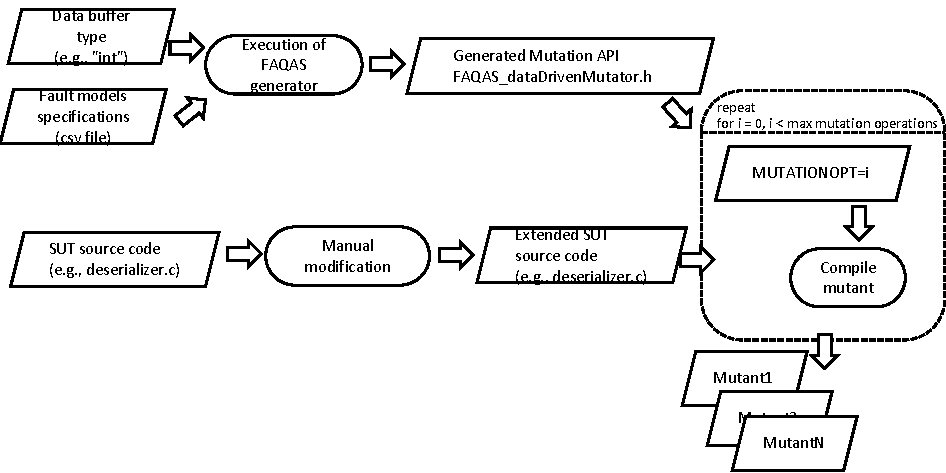
\includegraphics[width=14cm]{images/dataDrivenBufferProcess}
      \caption{Data-driven mutation process for buffered data: generation of one mutant for each mutation operation.}
      \label{fig:DataDrivenBufferProcess}
\end{figure}~\begin{figure}[h]
  \centering
    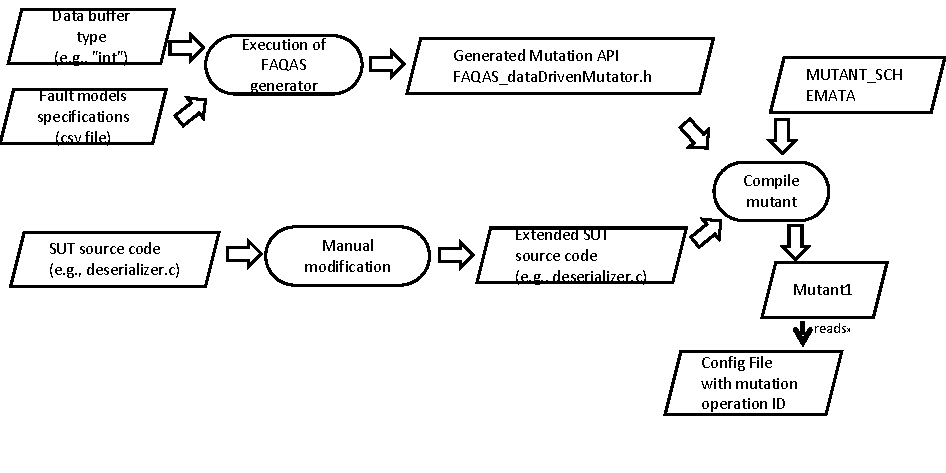
\includegraphics[width=14cm]{images/dataDrivenBufferProcess_ALT}
      \caption{Data-driven mutation process for buffered data: mutant schemata (i.e., generation of a single mutant). The mutation operation to perform is selected using an ID specified in a configuration file.}
      \label{fig:DataDrivenBufferProcessALT}
\end{figure}

\clearpage


The code that invokes the automatically generated probe is manually inserted by the engineer as shown in Listing~\ref{probesExample}.
The logic of the mutation probes is predefined and shared by all the mutation probes. What determines the different behaviours is the fault model.
The definition of the fault model is automatically generated in a \EMPH{C struct} (see Listing~\ref{faultModelExample}). 
The backbone data structures are predefined an provided in Listing~\ref{faultModelStructure}.

The code of the mutation probe is shown in Listing~\ref{mutationProbe}. It works by identifying the data item to mutate, the mutation operator to apply, and the mutation operation to execute by invoking methods \EMPH{\_FAQAS\_selectItem},
\EMPH{\_FAQAS\_selectOperator}, and \EMPH{\_FAQAS\_selectOperation}, respectively. The implementation of these three methods is automatically generated based on the fault model definition file.
An example is shown in Listing~\ref{selectors}. The runtime behaviour depends on the variable \EMPH{MUTATION}, whose value depends on the option passed at compile time. 
The variable \EMPH{MUTATION} uniquely identifies an instance of a mutation operation.
% (i.e., a mutation operation that belongs to a mutation operator defined for a specific data item of the fault model).

% !TEX root =  ../MAIN.tex

\begin{minipage}{15cm}
\begin{lstlisting}[style=CStyle, caption=Example of a data-driven mutation probes., label=probesExample, mathescape=true]


int receiveData()
{

    std::vector<char> v = connectAndReceiveData(); //function that receives data

    //MANUALLY ADDED PROBE
    FaultModel *fm = _FAQAS_IfHK_FM();
    _FAQAS_mutate(v->data(),fm);
    //MANUALLY ADDED PROBE END


}
\end{lstlisting}
\end{minipage}



% !TEX root =  ../MAIN.tex

\begin{minipage}{15cm}
\begin{lstlisting}[style=CStyle, caption=Example of generated fault models in C., label=faultModelExample, mathescape=true]
#define SIZE_IfHK 4
#define SIZE_IfStatus 1


struct FaultModel* _FAQAS_IfHK_FM(){
FaultModel *fm = _FAQAS_create_FM(SIZE_IfHK);

fm->items[0].operators[0].type=BF;
fm->items[0].operators[0].min=0;
fm->items[0].operators[0].max=0;
fm->items[0].operators[0].state=-1;
fm->items[0].operatorsN=1;
fm->items[0].span=1;
fm->items[0].type=BIN;

fm->items[1].operators[0].type=VOR;
fm->items[1].operators[0].min=0;
fm->items[1].operators[0].max=5;
fm->items[1].operators[0].delta=1;
fm->items[1].operatorsN=1;
fm->items[1].span=1;
fm->items[1].type=INT;

fm->items[2].operators[0].type=BF;
fm->items[2].operators[0].min=0;
fm->items[2].operators[0].max=0;
fm->items[2].operators[0].state=-1;
fm->items[2].operatorsN=1;
fm->items[2].span=2;
fm->items[2].type=BIN;

fm->items[4].operators[0].type=BF;
fm->items[4].operators[0].min=0;
fm->items[4].operators[0].max=0;
fm->items[4].operators[0].state=-1;
fm->items[4].operatorsN=1;
fm->items[4].span=1;
fm->items[4].type=BIN;
return fm;
}
struct FaultModel* _FAQAS_IfStatus_FM(){
FaultModel *fm = _FAQAS_create_FM(SIZE_IfStatus);

fm->items[0].operators[0].type=BF;
fm->items[0].operators[0].min=0;
fm->items[0].operators[0].max=0;
fm->items[0].operators[0].state=-1;
fm->items[0].operatorsN=1;
fm->items[0].span=1;
fm->items[0].type=BIN;
return fm;
}
\end{lstlisting}
\end{minipage}



% !TEX root =  ../MAIN.tex

\begin{minipage}{15cm}
\begin{lstlisting}[style=CStyle, caption=Fault model data structures., label=faultModelStructure, mathescape=true]
#define MAX_OPS 10
#define ITEMS 10


int MUTATION=MUTATIONOPT;

enum DataType {
    INT,
    FLOAT,
    DOUBLE,
    BIN
};

enum MutationType{
    BF,
    IV,
    VOR,
    VAT,
    VBT,
    INV
};

int _FAQAS_mutated = 0;

struct MutationOperator {
    MutationType type;
    int min;
    int max;
    int delta;
    int state;
};

struct DataItem {
    DataType type;
    int span;
    int operatorsN;
    struct MutationOperator operators[MAX_OPS];
};

struct FaultModel {
    int itemsN;
    struct DataItem *items;
};

\end{lstlisting}
\end{minipage}



% !TEX root =  ../MAIN.tex

\begin{minipage}{15cm}
\begin{lstlisting}[style=CStyle, caption=Automatically generated selectors., label=selectors, mathescape=true]
int _FAQAS_selectItem(FaultModel *dm){
if ( MUTATION == 0 )
    return 0;
if ( MUTATION == 1 )
    return 1;
if ( MUTATION == 2 )
    return 1;
if ( MUTATION == 3 )
    return 2;
if ( MUTATION == 4 )
    return 4;
if ( MUTATION == 5 )
    return 0;
}
int _FAQAS_selectOperator(FaultModel *dm){
if ( MUTATION == 0 )
    return 0;
if ( MUTATION == 1 )
    return 0;
if ( MUTATION == 2 )
    return 0;
if ( MUTATION == 3 )
    return 0;
if ( MUTATION == 4 )
    return 0;
if ( MUTATION == 5 )
    return 0;
}
int _FAQAS_selectOperation(FaultModel *dm){
if ( MUTATION == 0 )
    return 0;
if ( MUTATION == 1 )
    return 0;
if ( MUTATION == 2 )
    return 1;
if ( MUTATION == 3 )
    return 0;
if ( MUTATION == 4 )
    return 0;
if ( MUTATION == 5 )
    return 0;
}
\end{lstlisting}
\end{minipage}



% !TEX root =  ../MAIN.tex

\begin{minipage}{15cm}
\begin{lstlisting}[style=CStyle, caption=Mutation API function., label=mutationProbe, mathescape=true]
int _FAQAS_mutate( int *data, FaultModel *fm ){
    if ( _FAQAS_mutated == 1 )
    return 0;

    if ( MUTATION == -1 )
    return 0;

    int pos = _FAQAS_selectItem(fm);
    int op = _FAQAS_selectOperator(fm);
    int opt = _FAQAS_selectOperation(fm);

    int valueInt;
    int valueBin;
    double valueDouble;


    //Load the data in the appripriate var
    if ( fm->items[pos].type == BIN ){
        valueBin = (int) data[pos];
    }
    if ( fm->items[pos].type == INT ){
        valueInt = (int) data[pos];
    }
    if ( fm->items[pos].type == DOUBLE ){
        valueDouble = (double) data[pos];
    }
...
    MutationOperator *OP = &(fm->items[pos].operators[op]);    
...     
        if ( OP->type == VOR ){
        if ( fm->items[pos].type == INT ){

            if ( opt == 0 ){
                valueInt = OP->min-OP->delta;
            } else if (opt == 1 ){
                valueInt = OP->max+OP->delta;
            } else {
                //ERROR
            }
            _FAQAS_mutated = 1;
        }

...

    }

...

    if ( _FAQAS_mutated != 1 ){
        return 0;
    }

    //
    //Store the data
    //
    //FIXME: handle span
    if ( fm->items[pos].type == INT ){
        data[pos] = valueInt;
    }
    if ( fm->items[pos].type == DOUBLE ){
        data[pos] = valueDouble;
    }
    if ( fm->items[pos].type == BIN ){
        data[pos] = valueBin;
    }
    
    ...

    
\end{lstlisting}
\end{minipage}




\subsubsection{Data Mutation Probes for ASN.1}
\label{sec:FAQASDataMutationProbesASN}

%\DONE{This section still needs to be written. We may put a sequence diagram that show that at the beginning the probe loads the info about the mutation operation instance to execute and execute it if feasible.}

%Fabrizio: I removed the picture because it does not help the reader
%\begin{figure}[tb]
%  \centering
%    \includegraphics[width=\textwidth]{images/DataDrivenASNProcess}
%      \caption{Data-driven mutation process for ASN.1 grammars.}
%      \label{fig:DataDrivenASNProcess}
%\end{figure}


After the generation of the extended ASN.1 source code according to the 
the fault model definition process provided in Figure~\ref{fig:ASN1ProbesGeneration}, 
\MREVISION{C-P-37}{the FAQAS framework will automatically modify the extended ASN.1 deserializer (or serializer) code to insert calls to the FAQAS mutation API.
Particularly, the framework will insert one 
invocation of the automatically generated FAQAS mutation API for each data type to be mutated.}
Listings~\ref{ASN_encode} shows an example of a probe added at the beginning of function \emph{TypeNested\_encode} to mutated the TypeNested data to be encoded by function \emph{TypeNested\_encode}.
Listings~\ref{ASN_decode} shows an example of a probe added 
at the end of function \emph{TypeNested\_decode}
to mutated the TypeNested data decoded by function \emph{TypeNested\_decode}.

The insertion of the probe in the serializer code is useful when the fault model is not modified by the engineer but simply includes the boundary values automatically generated by the FAQAS framework. 
This is useful to generate invalid data to be serialized and thus test the capability of the ASN.1 serializer to detect illegal values.

The insertion of the probe in the deserializer code is useful to simulate the generation of invalid data from a faulty component. This is useful when the fault model had been modified by the engineer to reflect possible non-nominal cases with values belonging to the legal value domain.

%Figure~\ref{fig:DataDrivenASNProcess} provides an overview of the mutation process followed by the ASN.1 data mutation functions.
%At runtime, for each mutation operator instance, a single probe will be enabled. 

Similarly to the case of data mutation for data buffers, each mutant can implement a single mutation operation instance or work as a mutant schemata where the mutation operation instance is selected at runtime, based on a configuration parameter. Each mutation operator instance is identified by a unique identifier. 


%Fabrizio: You never introduced E, its not a good example!
%A MOI represents the mutation to be applied. More specifically, it contains the data type name to be mutated, and an ID that represents the mutation operator to be applied, and under what conditions applies.

%For example Listing~\ref{ASN_mutations} shows two possible MOI probes for the E data type. 
%\texttt{E\_1} exercises a mutation for the E data type when the value of \texttt{pVal} is less than or equal to 255. If the condition is true, then the value is modified by replacing it for the MAX value (e.g., 255).
%Similarly, \texttt{E\_2} exercises the E data type when the value of \texttt{pVal} is equal to 1299. If the condition applies, then the value is replaced by $1299 + 1$ (e.g., VAT mutation operator).
%The mutation is saved after its execution, so it is not performed twice. 

% !TEX root =  ../MAIN.tex
\begin{minipage}{14cm}
\begin{lstlisting}[style=CStyle, caption=Example of data-driven mutation probe for ASN.1 that has been added to the encoding function., label=ASN_encode]
flag TypeNested_Encode(const TypeNested* pVal, BitStream* pBitStrm, int* pErrCode, flag bCheckConstraints)
{
    TypeNested_mutate(pVal);
    flag ret = TRUE;
...
}
\end{lstlisting}
\end{minipage}

\begin{minipage}{14cm}
\begin{lstlisting}[style=CStyle, caption=Example of data-driven mutation probe for ASN.1 that has been added to the decoding function., label=ASN_decode]
flag TypeNested_Decode(TypeNested* pVal, BitStream* pBitStrm, int* pErrCode)
{
    flag ret = TRUE;
...
        // mutation
        TypeNested_mutate(pVal);

        return ret  && TypeNested_IsConstraintValid(pVal, pErrCode);
}
\end{lstlisting}
\end{minipage}

%flag E_Decode(E* pVal, BitStream* pBitStrm, int* pErrCode)
%{
%    flag ret = TRUE;
%    *pErrCode = 0;
%    (void)pVal;
%    (void)pBitStrm;
%
%
%    (*(pVal))=5; ret = TRUE; *pErrCode = 0;
%
%    // Manually added probe 
%    E_mutate(pVal);
%    // Manually added probe END
%    return ret  && E_IsConstraintValid(pVal, pErrCode);
%}



Listing~\ref{ASN_mutations} shows three possible mutation operation instances for the \emph{TypeNested} data type configured according to the fault model shown in Listing~\ref{asnXMLUpdated}.
\texttt{TypeNested\_1} applies the VAR operator,
 \texttt{TypeNested\_2} applies the VOR operator by setting the data value below the lower bound.
 \texttt{TypeNested\_3} applies the VOR operator by setting the data value above the upper bound.
% !TEX root =  ../MAIN.tex

\begin{lstlisting}[style=CStyle, caption=Example of automatically generated ASN.1 data-driven mutation operations., label=ASN_mutations]
// max E OR 1st operand constraint
if ( strcmp(buf,"E_1") ) {                                                  
	if ((*pVal) <= 255UL) {                                                                                                               
	    printf("%lu\n", *pVal);

	    if (*pVal != 255UL) {
	        *pVal = 255UL;
	        save_mutation();

	        return;
	    }           
	}       
}

// n+1 E 2nd operand constraint
if ( strcmp(buf, "E_2") ) {
    if ((*pVal) == 1299UL) {                                                                                                              
        printf("%lu\n", *pVal);

        *pVal = 1299UL + 1UL;
        save_mutation();
        return;
    }       
} 
\end{lstlisting}


\clearpage
\subsection{Test suite execution}
\label{sec:mutantsExecution}

During data mutation, the test suite is executed a number of times that depends on a stopping criterion chosen by the engineer. We foresee two possible stopping criteria (1) every test case is executed with every data mutation operation (hereafter, \INDEX{test coverage stopping criterion})
%, (2) exercise each data fault class (hereafter, fault coverage stopping criterion)
, and (2) a sample of the available data mutation operations is executed with every test case (hereafter, \INDEX{sampling stopping criterion}).

% !TEX root =  ../Main.tex

%\newcommand{\INDA}{10}
%\newcommand{\INDB}{15}
%\newcommand{\INDC}{5}

%\vspace{-3mm}
\begin{figure}[tb]

\begin{algorithmic}[1]

%\footnotesize
\scriptsize
\Require \emph{EMOS}, set of SUT executables, each one implementing one mutation operation (EMO)
\Require \emph{TS}, the test suite of the SUT
% (source inputs, follow-up inputs, output data).


\State \hspace{5 mm} \textbf{for each} $t$ in $TS$ \label{alg:prioritize:prel}
\State \hspace{10 mm} \textbf{execute} $t$ to track the data items exercised by t

\State \textbf{for each} $EMO$ in $EMO$ \label{alg:dataProcess:repeat}
\State \hspace{5 mm} \textbf{for each} $t$ in $TS$ \label{alg:prioritize:t}
\State \hspace{10 mm} \textbf{if} $t$ contains a data item that can be mutated with $EMO$ \label{alg:prioritize:cove}
\State \hspace{15 mm} \textbf{execute} $t$ with $EMO$
\State \hspace{15 mm} \textbf{if} $t$ fails or invalid data detected
\State \hspace{\INDB mm} \textbf{break} \label{alg:prioritize:stop}



\end{algorithmic}
\vspace{-3mm}
\caption{Algorithm for executing data-driven mutation testing with test coverage stopping criterion}
%\vspace{-0.2cm}
\label{alg:dataProcess}
\end{figure}




Figure~\ref{alg:dataProcess} shows how the data mutation process should be iterated with
 the \EMPH{test coverage stopping criterion}. 

Line~\ref{alg:dataProcess:prel} in Figure~\ref{alg:dataProcess} shows that the test suite is executed first just to track the data items exchanged during each test case execution. This is done using a mutated executable configured to simply track such information. It enables us to determine which test cases exercise the data items targeted by a specific mutation operation instance and thus speed-up the test execution process.

Then, for each mutation operation instance (Line~\ref{alg:dataProcess:repeat}), we execute every test case of the test suite (Line~\ref{alg:dataProcess:execute}), if the test case exercises the data item targeted by the mutation operation (Line~\ref{alg:dataProcess:cover}).
 The iterated execution can be stopped in advance if one of the test cases kills the mutant, i.e., it fails or detects the presence of invalid data and triggers a fault tolerant mechanism (Line~\ref{alg:dataProcess:stop}).
 
We can configure the data mutation API to inject a single data fault per execution or to mutate all the data items that can be targeted by the mutation operation instance (this is useful, for example, to simulate a bit that is always flipped because of a hardware fault).
 
The mutation algorithm can either mutate the first mutable data item observed or randomly decide whether to mutate the mutable data item. The second case enables the mutation of data items exchanged after long components interactions. However, it requires the repeated execution of a test case in case the mutation has not been performed but a data item could have been mutated. 


\newcommand{\ONMO}{\mathit{overall}\ \# \mathit{of}\ \mathit{mutation} \ \mathit{operation} \ \mathit{instances}}
\newcommand{\NMOA}{\# \mathit{of}\ \mathit{mutation} \ \mathit{operation}\ \mathit{instances} \ \mathit{applied}}


The outcome of the test execution is the $\ONMO$ (ONMO), the \\
$\NMOA$ (NMOA), and the $\# \ \mathit{of}\ \mathit{killed} \ \mathit{mutants}$ ($c_{\mathit{KILL}}$). They are used to compute the mutation score (see Section~\ref{sec:analyzeResults}).

The $\# \ \mathit{of}\ \mathit{killed} \ \mathit{mutants}$ corresponds to the number of \emph{mutants} that had been killed by at least one test case (Line~\ref{alg:dataProcess:kill}). A mutant is killed if the test case fails or if a redundancy mechanisms has been activated to handle the mutated data. To discover killed mutants it might be necessary to integrate automated solutions that, in addition to determine if a test case fails, determine if a redundancy mechanism has been triggered by the SUT. \MREVISION{C-P-39}{Assuming that the triggering of a redundancy mechanisms logs information in a log file, these solutions can be implemented through simple shell scripts that parse the log file of the SUT. Otherwise, debuggers scripts may be used to log the triggering of such mechanisms.}

The $\ONMO$ correspond with the $\mathit{overall}\ \# \mathit{of}\ \mathit{mutants}$; indeed, we have one different mutant for each mutation operation instance to be performed. 

The $\NMOA$, (\INDEX{NMOA}) captures the number of distinct mutation operation instances that were performed at least once. The mutation testing API creates a specific log file (i.e., \emph{FAQAS.mutant.applied.txt}) to indicate that a mutation operation instance was applied during a test execution. The file should be deleted after the execution of a test case.

\CHANGEDNOV{With the \EMPH{sampling stopping criterion} we perform the same activities performed for the test coverage criterion except that the set of mutation operation instances to be performed is randomly sampled. 
We aim to support the same sampling strategies considered for code-driven mutation testing: \emph{proportional uniform sampling}, \emph{proportional method-based sampling},  \emph{uniform fixed-size sampling}, and \emph{uniform FSCI sampling}.
To avoid influencing sampling results based on available data (e.g., to avoid ignoring mutants for which data is not available), the approach should first determine the subset of mutation operation instances to apply and then perform data-driven mutation. This way we will ensure achieving objective O2. In the case of FSCI, since the number of mutants is decided at runtime, we should sort mutation operation instances in a random order, and then apply data-driven mutation till the FSCI stopping criterion is reached.}

%We aim to support 

\subsubsection{Analyze Results}
\label{sec:analyzeResults}

The output  of activity \emph{Analyze Results} (see Figure~\ref{fig:data:process}) is a mutation score that is based on
the percentage of mutants being killed and the percentage of mutation operators applied. 
The former enables data-driven mutation to achieve objective O1, the latter objective O2 (see Section~\ref{sec:dataProcess}). 
The \INDEX{mutation score} can be computed as the weighted average of the percentage of mutants being killed and the percentage of mutation operations applied, according to the following formula

\begin{equation}
Score=w_{O1} \frac{\# \ \mathit{of}\ \mathit{killed} \ \mathit{mutants}}{\mathit{overall} \# \mathit{of}\ \mathit{mutants}} + w_{O2} \frac{\# \mathit{of}\ \mathit{mutation} \ \mathit{operations} \ \mathit{applied}}{\mathit{overall} \# \mathit{of}\ \mathit{mutation} \ \mathit{operations}}
\label{f:mutation:score}
\end{equation}

Where $w_{O1}$ and $w_{O2}$ capture the importance of the objectives O1 and O2, respectively. We assume $w_{O1}$ + $w_{O2} = 1$. In case objective $w_{O1}$ and $w_{O2}$ have the same importance, they should be set to $0.5$. 
%In the case of safety-critical systems, the mutation score should be equal to 1.





%With the fault coverage stopping criterion the full test suite is executed multiple times till all the possible data fault classes had been injected at least once (for the full test suite).
%A data fault class is no longer injected after it has already been injected in a test case of the test suite.
%The mutation algorithm can either mutate the first mutable data item observed or randomly decide whether to mutate the mutable data item.
%The repeated execution of a test case is terminated after it has been executed once without identifying any mutable data item.





\clearpage
\section{Test Suite Augmentation} % (fold)
\label{sec:data:test_suite_augmentation}


The test suite augmentation process concerns the definition of additional test cases to increase the mutation score.
It consists of four activities \emph{Identify Test Inputs}, \emph{Generate Test Oracles}, \emph{Execute the SUT}, \emph{Fix the SUT}. 
Despite these activities match the ones performed in the case of code-driven mutation testing, they are triggered and implemented in a different manner, as described below.

In the presence of mutants not killed by test cases (i.e., when the \emph{\% of Mutants Killed} is not equal to 100\%), engineers are expected to improve the oracles of existing test cases. Indeed, the presence of mutants not killed by test cases indicates that the oracles of the test suite are not capable of detecting that the software is failing. 
Automated approaches for performing this activity in the presence of system or integration test suites are not available and thus it needs to be performed manually.

In the presence of operators not being applied (i.e., the \emph{\% of Operators Applied} is not equal to 100\%), engineers are expected to generate new test inputs for the SUT that enable the application of all the mutation operators. 
To this end we aim to rely on solutions based on static program analysis. 
However the methodology to adopt may vary based on the test objective and the system architecture. In Figure~\ref{fig:dataDrivenTestSuiteAugmentation}, we provide an overview of the method to adopt for the case of a producer-consumer architecture. To make the example more concrete, we assume that the system exchange data of type TypeNested defined by relying on the ASN.1 grammar (see Listings~\ref{asnXMLUpdated} and ~\ref{asnXMLUpdated}). 
If the objective of data-driven mutation testing is to assess the quality of the test cases implemented to verify the consumer component. 
Such test cases may consist of sending predefined data through a producer component and verify that the consumer generates the expected output. 
To perform data-driven mutation, we may rely on a probe installed on the deserializer component. 

\begin{figure}[h]
  \centering
    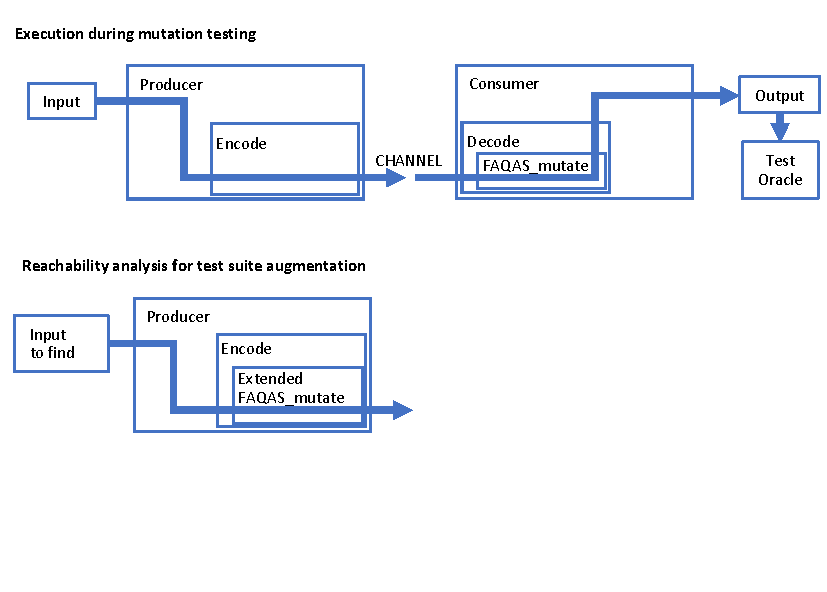
\includegraphics[width=14cm]{images/dataDrivenTestSuiteAugmentation}
      \caption{Data-driven Test Suite Augmentation by means of Static Analysis.}
      \label{fig:dataDrivenTestSuiteAugmentation}
\end{figure}

A \emph{\% of Operators Applied} not equal to 100\% indicates that the producer component does not produce all the required data types (e.g., TypeNested), which means that the functions that trigger the generation of such data types are not exercised. To enforce the generation of the required data types, we can augment the producer component by installing a mutation probe on the serializer interface (see Listing~\ref{ASN_encode}). In this case the probe should not be used to mutate the data but it should include assertions that enable reachability analysis. Listing~\ref{ASN_encodeReachable} shows an example where for each mutation operation implemented in the probe, we introduce an \emph{assert(false)} statement. Static analysis tools (i.e., CBMC and KLEE)  can then be used to find inputs that enable reaching any of these assertions from the entry point of the producer component. For each assertion, the static analysis component will look for an input of the entry point (e.g., the main function) that enables reaching the assertion, i.e., generate data that can be mutated according to the provided mutation operation. The identified inputs can then be used to augment the test suite.

% !TEX root =  ../MAIN.tex
\begin{lstlisting}[style=CStyle, caption=Example of data-driven mutation probe for ASN.1 that has been added to the encoding function., label=ASN_encodeReachable]
flag TypeNested_Encode(const TypeNested* pVal, BitStream* pBitStrm, int* pErrCode, flag bCheckConstraints)
{
    _FAQAS_TypeNested_cover(pVal);
    flag ret = TRUE;
...
}


void _FAQAS_TypeNested_cover(TypeNested *pVal) {

	// ALREADY_MUTATED is a global variable 
	// that traces if in the current execution we already performed data mutation
	if ( ALREADY_MUTATED ){
		return;
	}
	
	// intVal,VAT,1
	if ( ! has_been_mutated("TypeNested_1") ){
		// check that the value is not already 
		// what we want to generate

		if (pVal->intVal != 6 ){
			pVal->intVal = 6;
			assert(false);
			save_mutation("TypeNested_1");

			return;
		}
	}
	
	// int2Val,VOR,1
	if ( ! has_been_mutated("TypeNested_2") ){
		// check that the value is not already 
		// what we want to generate

		if (pVal->intVal != -1 ){
			pVal->intVal = -1;
			assert(false);
			save_mutation("TypeNested_2");

			return;
		}
	}

	// int2Val,VOR,2
	if ( ! has_been_mutated("TypeNested_3") ){

        printf("%lu\n", pVal -> intVal);

        if (pVal->intVal != 51){
        	    assert(false);	
            pVal->intVal = 51;
            save_mutation("TypeNested_3");

            return;
        }
    }


\end{lstlisting}



%flag E_Decode(E* pVal, BitStream* pBitStrm, int* pErrCode)
%{
%    flag ret = TRUE;
%    *pErrCode = 0;
%    (void)pVal;
%    (void)pBitStrm;
%
%
%    (*(pVal))=5; ret = TRUE; *pErrCode = 0;
%
%    // Manually added probe 
%    E_mutate(pVal);
%    // Manually added probe END
%    return ret  && E_IsConstraintValid(pVal, pErrCode);
%}


%For example, in the case of the example in Figure~\ref{fig:DataDrivenSimpleExample}, engineers would need to implement test cases that trigger the exchange of \emph{DataMessages}.
%Fully automated approaches to generate test cases for data-driven mutation testing are unavailable; however, techniques that generate input data from scratch~\cite{gligoric2010test} or augment input data~\cite{DiNardo:TOSEM:2017} can be adopted. 
%Also, when the data used by test cases is generated by simulators, meta-heuristic search can be used to drive the generation of input data~\cite{Abdessalem:ICSE:2018}. 
%
%The execution of the SUT and the repair of the SUT are performed manually as in the case of code-driven data mutation.
%
%
%\TODO{Clarify if we generate test cases or not}
%
%Section~\ref{sec:testGenerationData} provides details about the existing solutions to  \emph{Identify Test Inputs} and \emph{Generate Test Oracles}.


% !TEX root = MAIN.tex
\clearpage
\section{Evaluation of State-of-the-art, Data-driven Mutation Testing Toolsets}
\label{sec:toolsComparisonDataDriven}

This section describes an evaluation we conducted to identify a data-driven mutation testing tool applicable to space context. In particular, we assessed the \INDEX{Peach Fuzzer toolset}.

% description of the toolset

% !TEX root = ../MutationTestingSurvey.tex

\begin{table}[h]
\begin{center}
\footnotesize
\CHANGEDTWO{
\begin{tabular}{|p{5cm}|p{9cm}|}
\hline
\textbf{Operator Name}&\textbf{Description}\\
\hline
ArrayVarianceMutator&Change the length of arrays. Given L the original length of the array, the length is changed in range L-N to L+N.\\
ArrayReverseOrderMutator&Reverse the order of an array.\\
ArrayRandomizeOrderMutator&Put array elements in random order.\\
DWORDSliderMutator&Slides a DWORD through the blob.\\
BitFlipperMutator&Flips a given \% of bits in blob. Default is 20\%.\\
BlobMutator&Randomly grows a Blob block or shrinks it.\\
DataTreeRemoveMutator&Remove nodes from data tree.\\
DataTreeDuplicateMutator&Duplicate a node's value starting at 2x through 50x.\\
DataTreeSwapNearNodesMutator&Swap the data of two nodes that are near each other in the data model.\\
NumericalVarianceMutator&Produce numbers that are defaultValue - N to defaultValue + N.\\
NumericalEdgeCaseMutator&Replace with random numbers of appropriate correct size.\\
FiniteRandomNumbersMutator&Produce a finite number of random numbers for each \emph{Number} element.\\
NumericalEvenDistributionMutator&Generate numbers evenly distributed through the total numerical space of the number range.\\
NullMutator&Does nothing, just test the data produced by the fuzzer.\\
PathValidationMutator&Does not mutate. Used to trace path of each test for path validation.\\
SizedVarianceMutator&Change the length of sizes to count - N to count + N.\\
SizedNumericalEdgeCasesMutator&Change the length of sizes to numerical edge cases.\\
SizedDataVarianceMutator& Change the length of sized data to count - N to count + N. Size indicator will stay the same.\\
SizedDataNumericalEdgeCasesMutator&Change the length of sizes to numerical edge cases.\\
StringCaseMutator&Change the case of a string.\\
UnicodeStringsMutator&Generate unicode strings.\\
ValidValuesMutator&Replace with random values other than the legal ones.\\
UnicodeBomMutator&Injects BOM markers into default value and longer strings.\\
UnicodeBadUtf8Mutator&Generate bad UTF-8 strings.\\
UnicodeUtf8ThreeCharMutator&Generate long UTF-8 three byte strings.\\
StringMutator&Generate a random unicode string, for each string node, one Node at a time.\\
XmlW3CMutator&Replace XML trees with invalid, non-well former, and valid (but random) XML trees.\\
PathMutator&Replace a path with an erroneous path generated according to 20 different rules.\\
HostnameMutator&Replace a hostname with an erroneous hostname generated according to 20 different rules.\\
IpAddressMutator&Replace an IP address with an erroneous IP address generated according to 20 different rules.\\
TimeMutator&Replace a time value with an erroneous value generated according to 3 different rules.\\
DateMutator&Replace a date with 60 predefined erroneous dates.\\ 
FilenameMutator&Replace a file name with an file name generated according to 10 different rules.\\
ArrayNumericalEdgeCasesMutator&This operator is not well documented in the source code of Peach.\\
BlobSpread&This operator is not well documented in the source code of Peach.\\
\hline
\end{tabular}
}
\end{center}
\caption{Mutation Operators for the opensource version of Peach~\cite{PeachMozilla}}
\label{table:PeachOperators}
\end{table}%

% !TEX root =  ../MAIN.tex

\begin{minipage}{15cm}
\begin{lstlisting}[language=XML, caption=Portion of a Peach data model., label=peach, mathescape=true]
<Number name="lfh_CompSize" size="32" endian="little" signed="false"/>
<Number name="lfh_DecompSize" size="32" endian="little" signed="false"/>
<Number name="lfh_FileNameLen" size="16" endian="little" signed="false">
    <Relation type="size" of="lfh_FileName"/>
</Number>
<Number name="lfh_ExtraFldLen" size="16" endian="little" signed="false">
    <Relation type="size" of="lfh_FldName"/>
</Number>
<String name="lfh_FileName"/>
<String name="lfh_ExtraField"/>
\end{lstlisting}
\end{minipage}



Peach~\cite{PeachMozilla,PeachFuzzer} is a fuzzing tool that relies on \INDEX{block models}~\cite{pham2016model,spike} to perform data mutations. In other words, Peach performs mutations by altering the data of an input according to a large, predefined set of rules. For example, Listing~\ref{peach} introduces a portion of a data model describing the properties of the Zip data format~\cite{zipformat}. 

Even though Peach is currently a proprietary software~\cite{PeachFuzzer}, the Mozilla Foundation maintains a community edition of the toolset~\cite{PeachMozilla}, the community edition implements basic features such as the fuzzing capabilities. The proprietary version of Peach instead provides features for automatic generation of test cases and detailed reports about the potential security threats of a software~\cite{PeachFuzzer}. The version we evaluated in this activity was the community edition provided by the Mozilla Foundation. We provide an overview of the mutation operators implemented by the Peach community edition in Table~\ref{table:PeachOperators}.

% what we did

In the assessment of Peach, we defined three criteria to understand its applicability to the space context software. The first criteria concerns assessing if the community edition of Peach does work and if it can be installed properly. The second criteria concerns its portability. Finally, the third criteria concerns assessing its compatibility with FAQAS case study systems.

Regarding the first criteria, we tested Peach by applying it to the \texttt{unzip} program, and zip file mutants with the fuzzing capabilities of Peach. For this objective we reproduced the steps indicated in~\cite{zipexample}. So, first, we generated a Peach Data Model for Zip data files, and then we specified a launcher that enables the complete mutation process.

Peach provides a monitoring infrastructure that enables the execution of the whole mutation process. The process consists of the following steps:
\begin{enumerate}
	\item Specifying the data model for the a data type into an XML file.
	\item Loading the data model into Peach.
	\item Generating a new mutant (i.e, a mutated input).
	\item Running the program taking as an input the generated mutant, and with the monitoring infrastructure enabled.
	\item If the program crashes the process is stopped.
	\item If the program does not crashes, the process goes back to step 3, performing a new mutation.
\end{enumerate}

In particular, we were able to generate mutants for the Zip data format, but we could not run the monitoring infrastructure since it had dependencies with graphical environments that prevent us to execute it properly.

Regarding the second criteria, and specifically its portability. We seek to integrate it into the case studies as a component of their software to mutate data once it is sent, basically the idea would be to intercept the methods that exchange data, and apply Peach directly to the variable containing the data.
During the evaluation, we discovered that Peach -mainly implemented in Python- can be used as a Python library, and that this library can be invoked to generate multiple mutants in a off-line mode.

% why it was discarded

Regarding the third criteria and its compatibility with our case studies, we conclude that its integration with embedded systems is unlikely to work, mainly because of the characteristics of our case study systems.
For example, the ESAIL case study system runs within a real-time operative system (i.e., RTEMS by Edisoft) that does not possess a filesystem. Therefore, integrating Peach into ESAIL is not feasible because it might affect the real-time performance of the application, and also because it will be necessary to implement a solution to port the Peach toolset into the ESAIL infrastructure.


\subsection{Empirical Evaluation Planning}
\label{sec:codemutation:evaluation}

\STARTCHANGEDNOV

The project will include empirical evaluation sessions with the case study systems that aim to address the following research questions:

\begin{itemize}

    \item[RQ1] \emph{Are data-driven mutation cost affordable in space context?} This research question aims to determine if data-driven mutation testing is feasible in terms of costs related to the set-up of the system.
    
        \item[RQ2] \emph{Does data-driven mutation scale in space context?} Given the large quantity of data exchanged by space software components, there is a risk that data-driven mutation require the execution of a large number of test cases. This research question aims to determine if data-driven mutation testing can scale up.
        
                \item[RQ3] \emph{How does data-driven mutation compare to code-driven mutation?} This research question aims to compare the results obtained with code-driven and data-driven test suite assessment. We are interested in answering the following subquestions: (RQ3.a) Do test cases that kill code-driven mutants tend kill also data-driven mutants? (RQ3.b) What type of mutants generated by data-driven mutation are not detected by means of code-driven mutants? (RQ3.b) Is it possible to find a relation between the mutation scored computed with data-driven  and code-driven mutation?
                
                \item[RQ4] \emph{To what extent equivalent and redundant mutants affect data-driven mutation?} We aim to investigate how likely data-driven mutants are affected by the presence of equivalent and redundant mutants.
                
                                \item[RQ5] \emph{Does mutants sampling lead to accurate results in the case of data-driven mutation testing?} This research question investigates if mutants sampling is accurate also in the case of data-driven mutation testing. 
                                
                                                 \item[RQ6] \emph{How do mutants sampling approaches compare in terms of performance?} We aim to determine which mutants sampling strategy reduces most the data-driven mutation testing execution time.                
                
                 \item[RQ7] \emph{Is it feasible to apply reachability analysis to automatically generate inputs that kill data-driven mutants?} This research question aims to evaluate, on a subset of the case study systems, if static analysis is a viable solution to generating test cases that kill data-driven mutants. We aim to address the following subquestions: (RQ7.a) Can static analysis generate inputs that trigger the mutants? (RQ7.b) Are the generated inputs valid (i.e., do they lead to valid executions or are discarded by the software)? 
    
    \end{itemize}
    
\ENDCHANGEDNOV    
